\documentclass[english]{pkupaper}

\usepackage{lipsum}
\usepackage{essay-def}
\usepackage{clrscode}
\usepackage{appendix}
\usepackage{mathrsfs}
\newcommand{\ind}{\ \ \ }
\newenvironment{eqt}{\begin{equation}\begin{aligned}}{\end{aligned}\end{equation}}
\usepackage{indentfirst}
\usepackage{algorithm}
\usepackage{algorithmic}
\usepackage{multirow}
\usepackage{makecell}
\renewcommand{\algorithmicrequire}{\textbf{Input:}}
\renewcommand{\algorithmicensure}{\textbf{Output:}}

\newcommand{\titlemark}{Final Report: Algorithms for large-scale optimal transport}

\DeclareRobustCommand{\authorthing}{
\begin{tabular}{cc}
汪祎非\thanks{The authors are arranged lexicographically.} & 朱峰\thanksmark{1} \\
1500010611 & 1600010643 
\end{tabular}
}
\title{\titlemark}
\author{\authorthing}
\date{}
\bibliography{DeepL}
\begin{document}
\maketitle
\section*{Statement}
The main content of this project is not used as course project or assignment in other courses.

\section{Introduction}
According to \cite{COT}, optimal transport is a mathematical gem at the interface between probability, analysis and optimization. The theoretical importance of OT is that it defines a metric between probability distributions, namely, Wasserstein metric. It reveals a canonical geometric structure with rich properties to be exploited.  The earliest contribution to OT originated from Monge in 18th century. Kantorovich rediscovered it under a different formalism, namely the Linear Programming formulation of OT. With the development of scalable solvers, OT is widely applied to problems in imaging sciences(color and texture processing), computer vision and machine learning(regression).

In this report, we focus on the LP formulation and the Entropy Regularization of optimal transport. Our report is organized as follows. In Section \ref{sec:2}, we propose three first-order methods and introduce Bregman ADMM. In Appendix we also introduce a splitting method with penalty functions. The Entropy Regularization of optimal transport and Sinkhorn's algorithm is presented in Section \ref{sec:3}. We further propose an improvement of Sinkhorn's algorithm and ADMM for Entropy Regularization. Section \ref{sec:4} presents five datasets and contains comprehensive numerical experiments. In Section \ref{sec:5}, we conclude our work. 

Question 1(a) is answered in Section 4.2. Question 1(b) is answered in Section 2. Question 2 is answered in Section 3. The numerical results of all questions are provided in Section 4. The division of our work is listed in Acknowledgement (in the end of our report).

\section{First Order Methods for Optimal Transport}
\label{sec:2}
We consider to solve the standard form of Linear Programming (LP).
\begin{equation}
\label{lp}
\begin{aligned}
\min\limits_{\pi\in\mbR^{m\times n}}&\sum_{i=1}^m\sum_{j=1}^nC_{i,j}\pi_{i,j}\\
s.t.&\sum_{j=1}^n\pi_{i,j}=\mu_i, \, \forall i=1, 2, \dots m\\
&\sum_{i=1}^m\pi_{i,j}=\nu_j , \, \forall j=1, 2, \dots n\\
&\pi_{i,j}\geqslant0 
\end{aligned}
\end{equation}
To ensure that the feasible set for problem \ref{lp} is non-empty, we assume that $\mu_i\geqslant 0, \nu_j\geqslant0$ and $\sum_{i=1}^m\mu_i=\sum_{j=1}^n\nu_j$. Without loss of generality, we further assume $C_{i,j}\geqslant 0$ and $\sum_{i=1}^m\mu_i=\sum_{j=1}^n\nu_j=1$. Else we could add a positive constant on $C_{i, j}$ and divide $\mu_i$ and $\nu_j$ by $\sum_{i=1}^m\mu_i=\sum_{j=1}^n\nu_j$.

\subsection{ADMM: Complete Splitting}
\subsubsection{ADMM for primal}
We introduce a new variable $\tilde \pi \in \mbR^{m\times n}$ and split the constraints into two sets $\{\pi\in \mbR^{m\times n}| \sum_{j=1}^n\pi_{i,j}=\mu_i, \sum_{i=1}^m\pi_{i,j}=\nu_j\}$ and $\{\tilde\pi\in \mbR^{m\times n}|\tilde\pi\geq0\}$. Then we rewrite the LP problem \ref{lp} in the following form,
\begin{equation}
\label{new_lp}
\begin{aligned}
\min\limits_{\pi\in\mbR^{m\times n}}&\sum_{i=1}^m\sum_{j=1}^nC_{i,j}\pi_{i,j}\\
\text{s.t.}&\sum_{j=1}^n\pi_{i,j}=\mu_i,\quad \sum_{i=1}^m\pi_{i,j}=\nu_j\\
&\pi_{i,j} = \tilde\pi_{i,j}, \quad \tilde\pi_{i,j}\geqslant0 
\end{aligned}
\end{equation}
Then we write down its augmented Lagrangian function as follows,
\begin{eqt}
&L_t(\pi, \tilde{\pi}, \gamma, \lambda, \omega) \\
= &  \sum_{i, j}C_{i,j}\pi_{i,j} + \sum_{i}\gamma_i(\mu_i-\sum_{j}\pi_{i,j}) + \sum_{j}\lambda_j(\nu_j-\sum_i\pi_{i,j}) + \sum_{i, j}\omega_{i,j}(\tilde{\pi}_{i,j}-\pi_{i,j}) \\
&+ \frac{t}{2}\left(\sum_{i}(\mu_i-\sum_{j}\pi_{i,j})^2 + \sum_{j}(\nu_j-\sum_{i}\pi_{i,j})^2 + \sum_{i, j}(\tilde{\pi}_{i,j}-\pi_{i,j})^2\right)
\end{eqt}
where $\gamma\in\mathbb{R}^{m\times 1}, \lambda\in\mathbb{R}^{1\times n}, \omega\in\mathbb{R}^{m\times n}, \tilde{\pi}\in\mathbb{R}^{m\times n}, \tilde{\pi}_{i,j}\geqslant 0$. 

For the update of $\pi_{i,j}$, since $L$ is strongly convex with $\pi_{i,j}$, we set $\frac{\partial L}{\partial \pi_{ij}}$ to zero and yields
\begin{eqt}
\pi_{i,j} + \sum_{k}\pi_{i,k} + \sum_{k}\pi_{k,j} = \frac{1}{t}(\gamma_{i}+\lambda_{j}+\omega_{i,j}-c_{i,j}) + \mu_{i} + \nu_{j} + \tilde{\pi}_{i,j}\triangleq x_{i,j} \label{pi}
\end{eqt}
Though a bit complicated, (\ref{pi}) can be solved in closed form, 
\begin{eqt}
\label{upd_pi}
\pi_{i,j} \gets x_{i,j} & - \frac{1}{m+1}\left(\sum_kx_{k,j} - \frac{1}{m+n+1}\sum_{k, l}x_{k,l}\right)
\\& - \frac{1}{n+1}\left(\sum_kx_{i,k}-\frac{1}{m+n+1}\sum_{k, l}x_{k,l}\right)
\end{eqt}

To update $\tilde{\pi}_{i,j}$, it's easy to compute that
\begin{eqt}
\label{upd_pit}
\tilde{\pi}_{i,j} \gets (\pi_{i,j}-\frac{\omega_{i,j}}{t})_+
\end{eqt}

For the update of multipliers, we have 
\begin{eqt}
& \gamma_{i} \gets \gamma_i + t(\mu_i - \sum_k\pi_{i,k}) \\
& \lambda_{j} \gets \lambda_j + t(\nu_j - \sum_k\pi_{k,j}) \\
& \omega_{i, j} \gets \omega_{i, j} + t(\tilde{\pi}_{i, j} - \pi_{i, j}) \label{multiplier}
\end{eqt}

We thus can obtain the following Algorithm \ref{alg:ADMM}.

\begin{algorithm}
\caption{ADMM for Optimal Transport}
\label{alg:ADMM}
\begin{algorithmic}[1]
\REQUIRE {$C\in\mbR^{m\times n}$, $\mu\in\mbR^m$, $\nu\in\mbR^n$, $t\in \mathbb{R}^+$}
\STATE $\pi, \tilde{\pi}, \gamma, \lambda, \omega\gets 0$
\WHILE {\text{not converge}} 
	\STATE Update $\pi$ by \ref{upd_pi}
	\STATE Update $\tilde\pi$ by \ref{upd_pit}
	\STATE Update $\gamma, \lambda, \omega$  by \ref{multiplier}
\ENDWHILE
\RETURN $\pi$
\end{algorithmic}
\end{algorithm}

\subsubsection{ADMM for dual}

We also derive and implement an ADMM for dual problem of Optimal Transport. The Lagrangian of \ref{lp} is given by
\begin{eqt}
&\min_{\pi}\max_{\omega\geqslant 0, \gamma, \lambda}L(\pi, \gamma, \lambda, \omega) \\
= &  \sum_{i, j}C_{i,j}\pi_{i,j} - \sum_i\gamma_i(\mu_i-\sum_{j}\pi_{i,j}) - \sum_j\lambda_j(\nu_j-\sum_i\pi_{i,j}) - \sum_{i, j}\omega_{i,j}\pi_{i,j}\label{primallagrangian}
\end{eqt} 

However, the first two constraints in \ref{new_lp} are linearly dependent. More rigorously, one constraint can be removed since $\sum_{i=1}^m\mu_i = \sum_{j=1}^n\nu_j$. Thus, we impose another constraint on the dual variables in \ref{primallagrangian}, namely, $\lambda_n=0$. 

Calculating $\max_{\omega\geqslant 0, \gamma, \lambda}\min_{\pi_{i, j}}L(\pi, \gamma, \lambda, \omega)$ yields the dual problem
\begin{eqt}
\max_{\gamma, \lambda}&\ -\sum_i\gamma_i\mu_i - \sum_j\lambda_j\nu_j \\
\text{s.t.}&\ C_{i, j}+\gamma_i+\lambda_j\geqslant 0 \\
&\ \lambda_{n} = 0 \label{dual}
\end{eqt}
which is equivalent to 

\begin{eqt}
\min_{\gamma, \lambda}&\ \sum_i\gamma_i\mu_i + \sum_j\lambda_j\nu_j \\
\text{s.t.}&\ C_{i, j}+\gamma_i+\lambda_j\geqslant 0 \\
&\ \lambda_n=0 \label{dual2}
\end{eqt}

Similar to that in Section (2.1.1), we introduce a new variable $ z_{i, j} \in \mbR^{m\times n}$ and split the constraints into two sets $\{\gamma\in \mbR^{m\times 1}, \lambda\in \mbR^{1\times n}| C_{i, j}+\gamma_i+\lambda_j=z_{i, j}\}$ and $\{z_{i, j}\in \mbR^{m\times n}|z_{i, j}\geqslant0\}$. We can now write down its augmented Lagrangian function,
\begin{eqt}
L_t(\gamma, \lambda, \omega, z, \tilde z) = &\sum_i\gamma_i\mu_i + \sum_j\lambda_j\nu_j + \omega_{i, j}(C_{i, j}+\gamma_i+\lambda_j-z_{i, j}) \\&+ \frac{t}{2}\sum_{i, j}(C_{i, j}+\gamma_i+\lambda_j-z_{i, j})^2
\label{alf-dual}
\end{eqt}
where $\gamma\in\mathbb{R}^{m\times 1}, \lambda\in\mathbb{R}^{1\times n}, \omega\in\mathbb{R}^{m\times n}, z\in\mathbb{R}^{m\times n}, z_{i,j}\geqslant 0, \lambda_n=0$. In LP problems, ``dual of dual" is primal, and $\omega$ has direct relation with $\pi$. In fact, if we ignore the quadratic term in \ref{alf-dual}, we can find that $\omega = -\pi$. This imples that $-\omega$ can be interpreted as an approximation to $\pi$ in the primal problem.

For the update of $z_{i, j}$, we have
\begin{eqt}
z_{i, j}\gets \max\{C_{i, j}+\gamma_i+\lambda_j+\frac{\omega_{i, j}}{t}, 0\} \label{splitvarupdate}
\end{eqt}

For the update of $\gamma$ and $\lambda$, we set $\frac{\partial L}{\partial \gamma_i}$ and $\frac{\partial L}{\partial \lambda_j}$ to zero and yield
\begin{eqt}
n\gamma_i+\sum_j\lambda_j = \sum_jz_{i, j}-\sum_jC_{i, j}-\frac{1}{t}(\mu_i+\sum_j\omega_{i, j})&\triangleq a_i\ (i=1, ..., m)\\
m\lambda_j + \sum_i\gamma_i = \sum_iz_{i, j} - \sum_iC_{i, j} - \frac{1}{t}(\nu_j+\sum_i\omega_{i, j})&\triangleq b_j\ (j=1, ..., n-1) \label{equation}
\end{eqt}

Thanks for $\lambda_n=0$, \ref{equation} has a unique solution:
\begin{eqt}
&\gamma_i \gets \frac{1}{n}\left(a_i-\sum_ia_i+\sum_jb_j\right)\ (i=1, ..., m)\\
&\lambda_j \gets \frac{1}{m}\left(b_j - \frac{n}{m}\sum_jb_j+\frac{n-1}{m}\sum_ia_i\right)\ (j=1, ..., n-1). \label{dualupdate}
\end{eqt}

For the update of multipliers, it's easy to obtain that
\begin{eqt}
\omega_{i, j}\gets \omega_{i, j}+t(C_{i, j}+\gamma_i+\lambda_j-z_{i, j}). \label{multiplierupdate}
\end{eqt}

We thus can obtain the following Algorithm \ref{alg:ADMM-dual}.

\begin{algorithm}
\caption{ADMM for Dual of Optimal Transport}
\label{alg:ADMM-dual}
\begin{algorithmic}[1]
\REQUIRE {$C\in\mbR^{m\times n}$, $\mu\in\mbR^m$, $\nu\in\mbR^n$, $t\in \mathbb{R}^+$}
\STATE $\gamma, \lambda, \omega\gets 0$
\WHILE {\text{not converge}} 
	\STATE Update $\gamma, \lambda$ by \ref{dualupdate}
	\STATE Update $z$ by \ref{splitvarupdate}
	\STATE Update $\omega$  by \ref{multiplierupdate}
\ENDWHILE
\RETURN $-\omega$
\end{algorithmic}
\end{algorithm}

\subsection{ADMM: Simplex Splitting}
\label{sec:2.2}
We still focus on the primal problem, but this time, we utilize another splitting method. We rewrite the problem \ref{lp} as follows,
\begin{eqt}
\min_{\pi\in\mathbb{R}^{m\times n}}&\ \sum_{i=1}^m\sum_{j=1}^nC_{i, j}\pi_{i, j} \\
\text{s.t.}&\ \sum_{j}\pi_{i, j} = \mu_i,\ \sum_{i}\tilde{\pi}_{i, j} = \nu_j \\
&\ \pi_{i, j} = \tilde{\pi}_{i, j}\geqslant 0
\end{eqt}
The augmented Lagrangian function can be written as
\begin{eqt}
L_t(\pi, \tilde{\pi}, \omega) = & \sum_{i, j}C_{i, j}\frac{\pi_{i, j} + \tilde{\pi}_{i, j}}{2} + \sum_{i, j}\omega_{i, j}(\pi_{i, j} - \tilde{\pi}_{i, j}) + \frac{t}{2}\sum_{i, j}(\pi_{i, j}-\tilde{\pi}_{i, j})^2 \\
\text{s.t.}\ & \sum_{j}\pi_{i, j} = \mu_i,\ \pi_{i, j} \geqslant 0 \\
& \sum_{i}\tilde{\pi}_{i, j} = \nu_j,\ \tilde{\pi}_{i, j}\geqslant 0
\end{eqt} 

For update of $\pi$, we need to solve the following subproblem, i.e., the projection on a simplex,
\begin{eqt}
&\min_{\pi}\ \sum_{i, j}\left(\pi_{i, j} - \tilde{\pi}_{i, j}+\frac{1}{t}\left(\omega_{i, j} + \frac{C_{i, j}}{2}\right)\right)^2 \\
&\text{s.t.}\ \sum_{j}\pi_{i, j} = \mu_i, \ \pi_{i, j} \geqslant 0 \label{projpro}
\end{eqt}

From standard duality theory and with some calculation, we can derive that the solution must be the form 
\begin{eqt}
\pi_{i, j}\gets \max\{\tilde{\pi}_{i, j}-\frac{1}{t}\left(\omega_{i, j}+\frac{C_{i, j}}{2}\right)+\lambda_i, 0\} \triangleq \pi_{i, j}(\lambda_i) \label{projup}
\end{eqt}
where $\lambda_i$ is chosen such that 
\begin{eqt}
\sum_{j}\pi_{i, j}(\lambda_i) = \mu_i. \label{cst1}
\end{eqt}

Similarly, the update of $\tilde{\pi}$ can be written as
\begin{eqt}
\tilde{\pi}_{i, j} \gets \max\{\pi_{i, j}-\frac{1}{t}\left(\omega_{i, j}-\frac{C_{i, j}}{2}\right)+\tilde\lambda_j, 0\} \triangleq \tilde{\pi}_{i, j}(\tilde\lambda_j) \label{projup2}
\end{eqt}
where $\tilde\lambda_j$ is chosen such that 
\begin{eqt}
\sum_{i}\tilde\pi_{i, j}(\tilde\lambda_j) = \nu_j. \label{cst2}
\end{eqt}

We now briefly describe an algorithm mentioned in \cite{projection} to find the exact value of $\lambda$. For simplicity of statement, we consider the following problem, which is the canonical form of \ref{projpro},
\begin{eqt}
\min_{\mathbf{x}}&\ \frac{1}{2}\|\mathbf{x}-\mathbf{v}\|_2^2 \\
\text{s.t.}&\ \|\mathbf{x}\|_1 = z,\ \mathbf{x}\geqslant 0,
\end{eqt}
where $\mathbf{x}, \mathbf{v}\in\mathbb{R}^n$, $z\geqslant 0$. First, we sort $\mathbf{x}$ into descending order, namely
\begin{eqt}
y_1 \geqslant y_2 \geqslant ... \geqslant y_n. \label{descend}
\end{eqt}
Then we set 
\begin{eqt}
& \rho \gets \max\left\{j\in[n]: y_j - \frac{1}{j}\left(\sum_{r=1}^jy_r-z\right) > 0\right\} \\
& \lambda \gets \frac{1}{\rho}\left(z-\sum_{r=1}^\rho y_r\right) \\
& \mathbf{x} \gets \max\{\mathbf{x}-\lambda, 0\} \label{projupdate}
\end{eqt}
if $z>0$. If $z=0$, then $\mathbf{x}$ is automatically $\mathbf{0}$.

For multipliers, it's easy to have the following updates,
\begin{eqt}
\omega_{i, j} \gets \omega_{i, j} + t(\pi_{i, j} - \tilde\pi_{i, j}) \label{mult}
\end{eqt}
We thus have the following Algorithm \ref{alg:ADMM-split}:
\begin{algorithm}
\caption{ADMM for Primal of Optimal Transport: A second splitting method}
\label{alg:ADMM-split}
\begin{algorithmic}[1]
\REQUIRE {$C\in\mbR^{m\times n}$, $\mu\in\mbR^m$, $\nu\in\mbR^n$, $t\in \mathbb{R}^+$}
\STATE $\pi, \tilde{\pi}, \gamma, \lambda, \omega\gets 0$
\WHILE {\text{not converge}} 
	\STATE Update $\pi$ according to \ref{projup}, \ref{descend} and \ref{projupdate}
	\STATE Update $\tilde\pi$ according to  \ref{projup2}, \ref{descend}, and \ref{projupdate}
	\STATE Update $\omega$ by \ref{mult}
\ENDWHILE
\RETURN $\pi$
\end{algorithmic}
\end{algorithm}

\subsection{Bregman ADMM}
\cite{BADMM} proposes Bregman ADMM, which uses Bregman divergence to replace the penalty term in ADMM. Let $\phi: \Omega \to \mbR$ be a continuously differentiable and strictly convex function on the relative interior of the convex set $\Omega$. We define the Bregman divergence $B_\phi:\Omega\,\times \,\mathrm{relint} \, \Omega\to\mbR_+$ induced by $\phi$ as
\begin{equation}
B_\phi(x,y)=\phi(x)-\phi(y)-\la\nabla \phi(y),x-y\ra
\end{equation}
From the convexity of $\phi$, $B_\phi(x,y)\geqslant 0$ and the equality holds if and only if $x=y$. To solve the LP problem \ref{lp}, we consider to take $\phi(x)=\sum_{i}x_i\log(x_i)$. In this case, $B_\phi(x,y)=\mathrm{KL}(x,y)$ is the KL divergence between $x$ and $y$.

Similar to that in Section \ref{sec:2.2}, we introduce a new variable $\tilde \pi\in\mbR^{m\times n}$ to split the constraints into two simplex $S_\mu=\{\pi|\pi\geqslant0, \pi\mbone_n = \mu\}$ and $S_\nu=\{\tilde \pi |\tilde \pi\geqslant 0, \tilde \pi^T\mbone_m = \mu\}$. Then problem \ref{lp} can be written in the following form,
\begin{equation}
\left\{
\begin{aligned}
&\min\quad \la C, \pi\ra\\
&\mathrm{s.t.}\quad \pi\in S_\mu, \tilde \pi\in S_\nu, \pi=\tilde \pi
\end{aligned}
\right.
\end{equation}

We then introduce another variable $\sigma\in\mbR^{m\times n}$ for BADMM. Given $(\pi^{(l)},\tilde\pi^{(l)},\sigma^{(l)})$, we first update $\pi^{(l+1)}$ and $\tilde\pi^{(l+1)}$:
\begin{equation}
\label{badmm_pi_upd}
\pi^{(l+1)}=\arg\min\limits_{\pi\in S_\mu} \la C, \pi\ra+\la \tilde \sigma^{(l)}, \pi\ra+t \KL(\pi,\tilde\pi^{(l)})
\end{equation}
\begin{equation}
\label{badmm_pit_upd}
\tilde\pi^{(l+1)}=\arg\min\limits_{\tilde\pi\in S_\nu} \la \sigma^{(l)}, -\tilde\pi\ra+t \KL(\tilde\pi, \pi^{(l+1)})
\end{equation}
Both \ref{badmm_pi_upd} and \ref{badmm_pit_upd} have closed form solution
\begin{equation}
\label{badmm_pipit_upd}
\pi_{i,j}^{(l+1)}=\frac{\tilde\pi^{(l)}_{i,j}\exp(-\frac{C_{i,j}+\sigma_{i,j}^{(l)}}{t})}{\sum_{j=1}^n\tilde\pi^{(l)}_{i,j}\exp(-\frac{C_{i,j}+\sigma_{i,j}^{(l)}}{t})}\mu_i, \quad \tilde\pi_{i,j}^{(l+1)}=\frac{\pi_{i,j}^{(l+1)}\exp(\frac{\sigma_{i,j}^{(l)}}{t})}{\sum_{i=1}^m\pi_{i,j}^{(l+1)}\exp(\frac{\sigma_{i,j}^{(l)}}{t})}\nu_j
\end{equation}
We update $\sigma^{(l+1)}$ as
\begin{equation}
\label{badmm_sigma_upd}
\sigma^{(l+1)} = \sigma^{(l)} + t (\pi^{(l+1)}-\tilde\pi^{(l+1)})
\end{equation}
Then we get the following Bregman ADMM, Algorithm \ref{alg:BADMM}.

\begin{algorithm}
\caption{Bregman ADMM for Optimal Transport}
\label{alg:BADMM}
\begin{algorithmic}[1]
\REQUIRE {$C\in\mbR^{m\times n}$, $\mu\in\mbR^m$, $\nu\in\mbR^n$, $t>0$}
\STATE Initialize $\tilde\pi^{(0)}=\mu\nu^T$, set $\sigma^{(0)}=\mathbf{0}_{n\times m}$, $l=0$
\WHILE {\text{not converge}}
	\STATE Update $(\pi^{(l+1)},\tilde\pi^{(l+1)},\sigma^{(l+1)})$ by \ref{badmm_pipit_upd} and \ref{badmm_sigma_upd}, $l=l+1$
\ENDWHILE
\RETURN $\frac{\pi^{(l)}+\tilde\pi^{(l)}}{2}$
\end{algorithmic}
\end{algorithm}

\cite{BADMM} proves that when $m=n$, BADMM can be faster than ADMM by a factor of $O(n/ \log(n))$. 

\section{Entropy Regularization of Optimal Transport}
\label{sec:3}
\subsection{Background and Formulation}
\subsubsection{Kantorovich formulation of optimal transport}
\cite{COT} introduces the Kantorovich formulation of optimal transport (Kantorovich's relaxation). For two vectors $\mu\in\mbR^m$ and $\nu\in\mbR^n$, which satisfies $\mbone_n^T\mu=\mbone_m^T\nu$, we consider the following set of coupling matrices
\begin{equation}
U(\mu, \nu) \triangleq \left\{\pi\in\mbR^{m\times n}_+: \pi\mbone_n = \mu, \pi^T\mbone_m=\nu \right\}
\end{equation}
where we use the following matrix-vector notation
$$
\pi\mbone_n  = (\sum_j \pi_{i,j})_i\in\mbR^m, \quad \pi\mbone_m  = (\sum_i \pi_{i,j})_j\in\mbR^n,
$$

The Kantorovich's optimal transport problem reads
\begin{equation}
\label{equ:kot}
L_\mfc(\mu,\nu)\triangleq \min\limits_{\pi\in U(\mu, \nu)}\la C,\pi\ra\triangleq\sum_{i,j}C_{i,j}\pi_{i,j}
\end{equation}
Therefore, problem \ref{equ:kot} is equivalent to the standard form of LP \ref{lp}. 

\subsubsection{Entropy regularization}
For a coupling matrix $\pi \in U(\mu, \nu)$, the discrete entropy of $\pi$ is defined as
\begin{equation}
H(\pi)\triangleq-\sum_{i,j}\pi_{i,j}(\log(\pi_{i,j})-1)
\end{equation}
with an analogous definition for vectors, with the convention that $H(\pi) = -\infty$ if one of the entries $\pi_{i,j}$ is negative. Although discrete entropy is defined on matrices with positive entry, with $\lim\limits_{x\to0+}x(\log x-1)=0$, we can extend its definition to  matrices with non-negative entry. And we have
$$
H(\pi)=-\sum_{\pi_{i,j}\geqslant0}\pi_{i,j}(\log(\pi_{i,j})-1)
$$
Suppose $M=\min\{\|\mu\|_\infty, \|\nu\|_\infty\}$, then we have $\pi_{i,j}\leqslant\min\{\mu_i, \nu_j\}\leqslant M$. The function $H(\pi)$ is then $1/M$-strongly convex, because its Hessian is $\p^2H(\pi)=-\diag(1/\pi_{i,j})$. 

The idea of entropic regularization of optimal transport is to use $-H$ as a regularizing function to obtain approximate solutions to the Kantorovich's optimal transport problem \ref{equ:kot}. 

\begin{equation}
\label{equ:erot}
L^\epsilon_C(\mu,\nu)\triangleq \min\limits_{\pi\in U(\mu, \nu)}\la C,\pi\ra-\epsilon H(\pi)
\end{equation}

The convergence of the solution of that regularized problem towards an optimal solution of the original linear program has been studied by \cite{aaote}. 
\begin{proposition}[Convergence with $\epsilon$]
\label{sh_cvg}
The unique solution $\pi^\epsilon$ of \ref{equ:erot} converges to the optimal solution with maximal entropy within the set of all optimal solutions of the Kantorovich problem, namely
\begin{equation}
\label{sh_limit}
\pi^\epsilon\to\arg\min\limits_\pi\{-H(\pi): \pi\in U(\mu,\nu), \la\pi, C\ra=L_C(\mu,\nu)\}, \quad \epsilon\to0
\end{equation}
so that in particular
$$
L^\epsilon_C(\mu,\nu)\to L_C(\mu,\nu), \quad \epsilon\to0
$$
\end{proposition}
\begin{proof}
We consider a sequence $\{\epsilon_l\}$ such that $\epsilon_l\to0$ and $\epsilon_l>0$. We denote $\pi^l$ the solution to \ref{equ:erot} for $\epsilon=\epsilon_l$. Since $U(\mu,\nu)$ is bounded, we can extract a sequence (that we do not relabel for sake of simplicity) such that $\pi^l\to\pi^*$. Since $U(\mu, \nu)$ is closed, $\pi^*\in U(\mu,\nu)$. We consider any $\pi$ such that $\la C,\pi\ra=L_C(\mu,\nu)$. By the optimality of $\pi$ and $\pi^l$ for their respective optimization problem, we have
\begin{equation}
0\leqslant\la C, \pi^l\ra-\la C, \pi\ra\leqslant\epsilon_l(H(\pi^l)-H(\pi))
\end{equation}
Since $H$ is continuous, taking the limit $l\to\infty$ in this expression shows that $\la C, \pi^*\ra=\la C, \pi\ra$ so that $\pi^*$ is a feasible point of \ref{sh_limit}. Furthermore, we have $H(P^*)\geqslant H(P)$, which shows that $P^*$ is the solution to \ref{sh_limit}. By strict convexity of $-H$, the solution is unique and the whole sequence is converging. 
\end{proof}

The following figures \ref{gmm1} and \ref{gmm2} illustrates the impact of $\epsilon$ on the coupling $\pi$ between two Gaussian mixture models.
\begin{figure}[!htb]
\centering
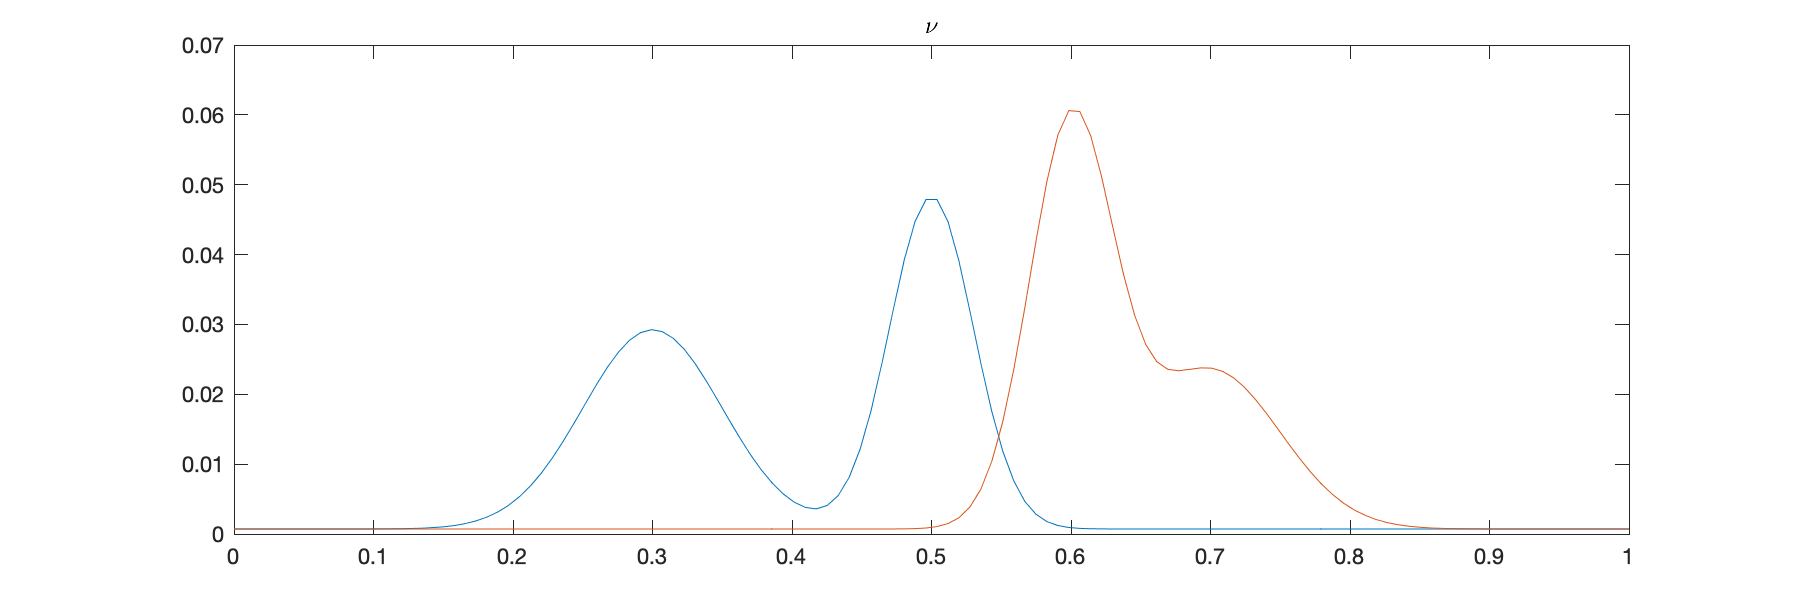
\includegraphics[width=12cm]{final/gmm1.png}
\caption{The probability distribution function of two Gaussian mixture models $G_1$ and $G_2$. $G_1$ (blue one) has mean $[0.3,0.5]$, variance $[0.05^2, 0.03^2]$ and component proportion $[0.5, 0.5]$; $G_2$ (red one) has mean $[0.6,0.7]$, variance $[0.03^2, 0.05^2]$ and component proportion $[0.6, 0.4]$. }
\label{gmm1}
\end{figure}

\begin{figure}[!htb]
\centering
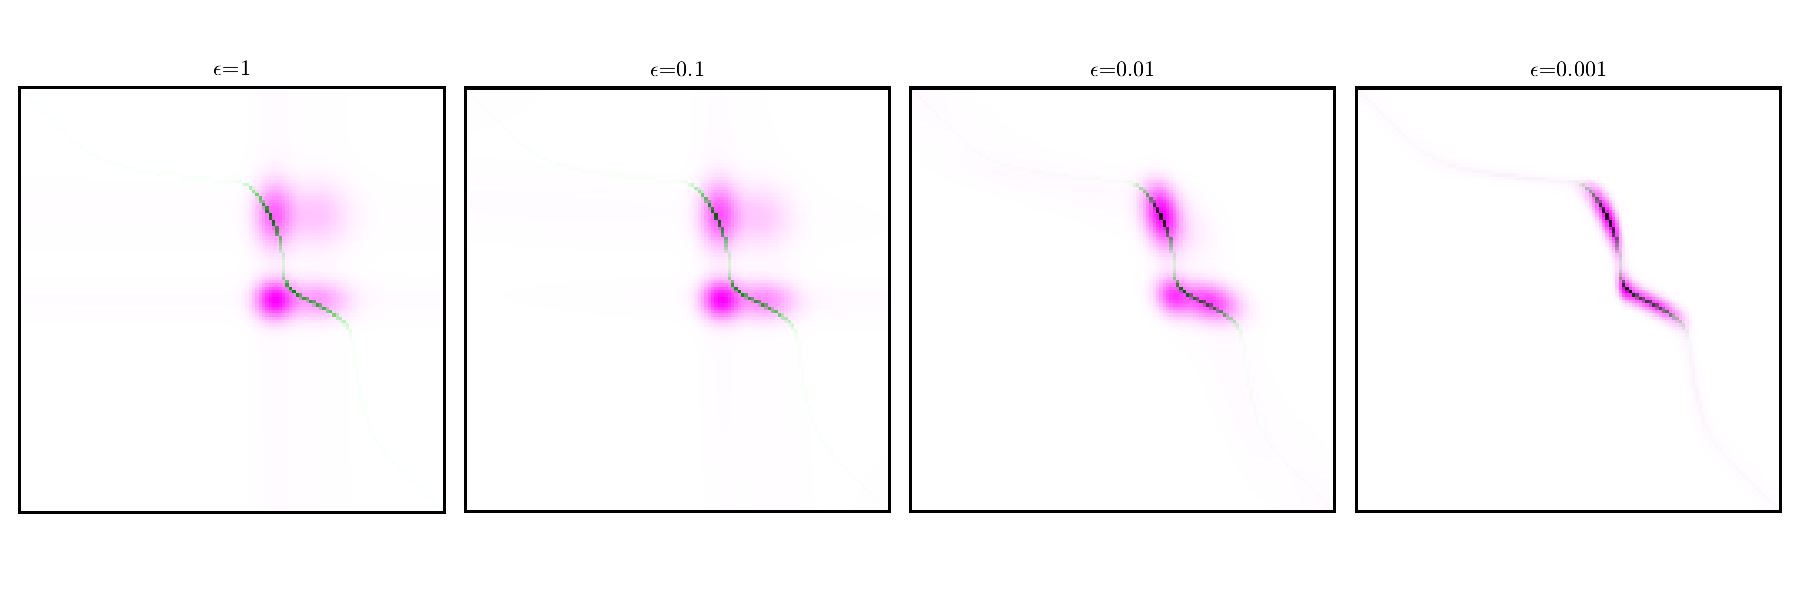
\includegraphics[width=12cm]{final/gmm2.png}
\caption{Impact of $\epsilon$ on the coupling between two gaussian mixture models \ref{gmm1}. From left to right, $\epsilon=1,0.1,0.01,0.001$. The purple one is the solution to the entropy regularized LP. The green one is the solution to the original LP.}
\label{gmm2}
\end{figure}

Define the Kullback-Leibler divergence between couplings as
$$
\mathrm{KL}(\pi|K)\triangleq\sum_{i,j}\pi_{i,j}\log(\frac{\pi_{i,j}}{K_{i,j}})-\pi_{i,j}+K_{i,j}
$$
We take $K^\epsilon_{i,j}\triangleq e^{-\frac{C_{i,j}}{\epsilon}}$, the Gibbs kernel associated to the cost matrix $C$. The unique solution $\pi^\epsilon$ of \ref{equ:erot} is a projection onto $U(\mu,\nu)$, namely
$$
\pi^\epsilon\triangleq\arg\min\limits_{\pi\in U(\mu,\nu)}\mathrm{KL}(\pi|K^\epsilon)
$$

\subsubsection{Formulation of the problem}
The optimization problem of the entropic regularization of optimal transport with parameter $\epsilon$ is given by:
\begin{equation}
\label{equ:kl}
\left\{
\begin{aligned}
&\min \, \la C,\pi\ra-\epsilon H(\pi)=\mathrm{KL}(\pi|K^\epsilon)\\
&\mathrm{s.t.}\, \pi\in U(\mu, \nu)
\end{aligned}\right.
\end{equation}
where $K^\epsilon_{i,j}= e^{-\frac{C_{i,j}}{\epsilon}}$.

\subsection{Sinkhorn's Algorithm}
We start with the following proposition. 

\begin{proposition}
\label{sh_basic}
The solution to \ref{equ:kl} is unique and has the form 
\begin{equation}
\label{equ:para}
\forall 1\leqslant i\leqslant m, 1\leqslant j\leqslant n, \quad \pi^\epsilon_{i,j}=a_iK^\epsilon_{i,j}b_j
\end{equation}
for two (unknown) scaling variable $(a,b)\in \mbR_+^m\times\mbR_+^n$.  
\end{proposition}

\begin{proof}
Introducing two dual variable $f\in\mbR^m, g\in\mbR^n$ for each marginal constraint. The Lagrangian of \ref{equ:kl} reads
$$
L(\pi,f,g)=\la\pi,C\ra-\epsilon H(P)-\la f, \pi\mbone_n-\mu\ra-\la g, \pi^T\mbone_m-\nu\ra
$$
The first order conditions yield
$$
\frac{\p L}{\p \pi_{i,j}}=C_{i,j}+\epsilon log(P_{i,j})-f_i-g_j=0
$$
This means that an optimal $\pi$ coupling to the regularized problem can be written as $P_{i,j}=e^{f_i/\epsilon}e^{-C_{i,j}/\epsilon}e^{g_j/\epsilon}$. Let $a=e^{f_i/\epsilon}, b= e^{g_j/\epsilon}$, then we have $$
\pi_{i,j}=a_iK^\epsilon_{i,j}b_j
$$
\end{proof}

This shows that the solution of \ref{equ:kl} has a specific form, which can be parameterized using $m+n$ variables.

The parameterization of the optimal solution in equation \ref{equ:para} can be written in the matrix form $\pi^\epsilon = \diag(a)K^\epsilon\diag(b)$. Then, $a,b$ must satisfies:
\begin{equation}
\diag(a)K^\epsilon\diag(b)\mbone_m=\mu, \quad \diag(a)K^T\diag(b)\mbone_n=\nu
\end{equation}
These two equations can be further simplified as
\begin{equation}
a\odot (K^\epsilon b)=\mu, \quad b\odot\left((K^\epsilon)^Ta\right)=\nu
\end{equation}
where $\odot$ corresponds to entry-wise multiplication of vectors. The Sinkhorn's algorithm iteratively update $a^{(l+1)}$ and $b^{(l+1)}$ by
\begin{equation}
\label{upd_sh}
a^{(l+1)}=\frac{\mu}{K^\epsilon b^{(l)}}, \quad b^{l+1}=\frac{\nu}{(K^\epsilon)^Ta^{(l+1)}}
\end{equation}
initialized with an arbitrary positive vector $b^{(0)}=\mbone_n$. The division operator used above between two vectors is to be understood entry-wise. The whole algorithm is given by:

\begin{algorithm}
\caption{Sinkhorn's algorithm}
\label{alg:sa}
\begin{algorithmic}[1]
\REQUIRE $\epsilon$, $C\in\mbR^{m\times n}$, $\mu\in\mbR^m$, $\nu\in\mbR^n$.
\STATE Start with $b^{(0)}=\mbone_n$, $l=0$
\STATE Calculate $K^\epsilon_{i,j}= e^{-\frac{C_{i,j}}{\epsilon}}$
\WHILE {\text{not converge}}
	\STATE Update $a^{(l+1)}$ and $b^{(l+1)}$ by \ref{upd_sh}, $l=l+1$
\ENDWHILE
\STATE $a=a^{(l)}, b=b^{(l)}$
\RETURN $\pi=\diag(a)K^\epsilon \diag(b)$
\end{algorithmic}
\end{algorithm}

This algorithm was originally introduced with a proof of convergence by \cite{sinkhorn}. For simplicity, we assume $m=n$. \cite{nltaa} showed that by setting $\epsilon=\frac{\tau}{4\log(n)}$, $O(\|C\|_\infty^3\log(n)\tau^{-3})$ Sinkhorn iterations (with an additional
rounding step to compute a valid coupling $\hat\pi\in U(\mu,\nu)$) are enough to ensure $\la \hat \pi, C\ra\leqslant L_C(\mu,\nu)+\tau$. This implies that Sinkhorn computes a $\tau$-approximate solution of the unregularized OT problem in $O(n^2\log(n)\tau^{-3})$ operations. The rounding scheme consists in, given two vectors $a\in\mbR^m, \, b\in\mbR^n$ to carry out the following updates:
$$
a'=a\odot \min\left(\frac{\mu}{a\odot(K^\epsilon b)},\mbone_m\right), \quad b'=b\odot \min \left(\frac{\nu}{b\odot((K^\epsilon)^Ta')},\mbone_n\right)
$$
$$
\Delta_\mu = \mu-a'\odot(K^\epsilon b'), \quad \Delta_\nu=\nu-b'\odot\left((K^\epsilon)^Ta'\right)
$$
$$
\hat \pi = \diag(a') K^\epsilon\diag (b')+\Delta_\mu\Delta_\nu^T/\|\Delta_\mu\|_1
$$
This yields a matrix $\hat\pi\in U(\mu,\nu)$ such that the $1$-norm of $\hat \pi -\diag(a) K^\epsilon\diag (b) $ is controlled by the marginal violations of $\diag(a)K^\epsilon\diag(b)$, namely
$$
\|\hat \pi -\diag(a) K^\epsilon\diag (b')\|_1\leqslant\|\mu-a\odot(K^\epsilon b)\|_1+\|\nu-b\odot\left((K^\epsilon)^Ta\right)\|_1
$$
In actual implementation, this step is crucial to decrease the violation of constraints. 

\subsection{Our proposed algorithm}
\subsubsection{Sinkhorn's algorithm with numerical stability and continuation strategy}
We denote $\|C\|_\infty=\max\limits_{i,j}|C_{i,j}|$. In actual implementation of Sinkhorn's algorithm \ref{alg:sa}, because we have $K^\epsilon_{i,j}=e^{-\frac{C_{i,j}}{\epsilon}}$, when $\epsilon$ is small, namely $\epsilon<\frac{\|C\|_\infty}{806}$, the largest entry of $K$ is smaller than $e^{-806}\approx 10^{-350}$. Most of the entry of $K^{\epsilon}$ would be rounded to $0$ because they are smaller than the smallest positive number that the computer can restore. If we want to calculate $K^\epsilon$, we would have a positive lower bound $\frac{\|C\|_\infty}{806}$ for $\epsilon$. This is not desired and it would make the result from proposition \ref{sh_cvg} meaningless.

We propose a numerical stable version of Sinkhorn's algorithm with no lower bound of $\epsilon$. A possible way to remove this lower bound of $\epsilon$ is to avoid directly calculating $K^\epsilon$ to update $a^{(l+1)}$ and $b^{(l+1)}$. Therefore, from the proof of proposition \ref{sh_basic}, we denote $a^{(l)}=e^{f^{(l)}/\epsilon}$, $b^{(l)}=e^{g^{(l)}/\epsilon}$, where $f^{(l)}\in R^m, g^{(l)}\in R^n$. Then, the update rule for $f^{(l+1)}$ and $g^{(l+1)}$ reads
\begin{equation}
\label{upd_sh_log}
f^{(l+1)}=\epsilon(\log(\mu)-\log(K^\epsilon e^{g^{(l)}/\epsilon})), \quad g^{(l+1)}=\epsilon(\log(\nu)-\log((K^\epsilon)^T e^{f^{(l+1)}/\epsilon})),
\end{equation}
Our motivation is to caculate $\log(K^\epsilon e^{g^{(l)}/\epsilon})$ and $\log((K^\epsilon)^T e^{f^{(l+1)}/\epsilon})$ in update rule \ref{upd_sh_log} in a numerically stable way. We start with the update of $f^{(l+1)}$. It is easy to verify that
$$
f^{(l+1)}_i = \epsilon \log(\mu_i)-\epsilon \log(\sum_{j=1}^ne^{(-C_{i,j}+g^{(l)}_j)/\epsilon})
$$
Directly calculating $\sum_{j=1}^ne^{(-C_{i,j}+g^{(l)}_j)/\epsilon}$ is dangerous because it might be rounded to $0$. Let $\hat f^{(l+1)}_i=\max_j\{-C_{i,j}+g^{(l)}_j\}$. Then, to update $f$ with numerical stability, we can update $f^{(l+1)}_i$ by
\begin{equation}
\label{sh_f_upd}
f^{(l+1)}_i = \epsilon \log(\mu_i)-\hat f^{(l)}_i-\epsilon \log(\sum_{j=1}^ne^{ (-C_{i,j}+g^{(l)}_j-\hat f^{(l)}_i)/\epsilon})
\end{equation}
Because $\sum_{j=1}^ne^{ (-C_{i,j}+g^{(l)}_j-\hat f^{(l)}_i)/\epsilon}\geqslant1$, to update $f^{(l+1)}$ in this way is safe. Actually, we use $\hat f_i^{(l)}/\epsilon+\log(\sum_{j=1}^ne^{ (-C_{i,j}+g^{(l)}_j-\hat f^{(l)}_i)/\epsilon})$ to calculate $\log(K^\epsilon e^{g^{(l)}/\epsilon})$.  Similarly, we let $\hat g^{(l+1)}_j=\max_i\{-C_{i,j}+f^{(l+1)}_i\}$, and update $g^{(l+1)}_j$ by
\begin{equation}
\label{sh_g_upd}
g^{(l+1)}_j = \epsilon \log(\nu_j)-\hat g^{(l+1)}_j-\epsilon \log(\sum_{i=1}^ne^{ (-C_{i,j}+f^{(l+1)}_i-\hat g^{(l+1)}_j)/\epsilon})
\end{equation}
In the end of the algorithm, we also use an additional rounding step to compute a valid coupling $\hat\pi$. Given two vectors $f\in\mbR^m, g\in\mbR^n$ and coupling matrix $\pi\in\mbR^{m\times n}$ with $\pi_{i,j}=e^{(f_i-C_{i,j}+g_j)/\epsilon}$, we compute $\hat\pi$ in the following way:
\begin{equation}
\label{add_coup}
\begin{aligned}
&\hat f_i=\max_j\{-C_{i,j}+g_j\}, \quad f'_i=f_i+\min\{\epsilon(\log(\mu_i)-\sum_{j=1}^ne^{ (-C_{i,j}+g_j-\hat f_i)/\epsilon})-\hat f_i-f_i,0\}\\
&\hat g_j=\max_i\{-C_{i,j}+f'_i\}, \quad g'_j=g_j+\min\{\epsilon(\log(\nu_j)-\sum_{i=1}^me^{ (-C_{i,j}+f'_i-\hat g_j)/\epsilon})-\hat g_j-g_j,0\}\\
&\hat f'_i=\max_j\{-C_{i,j}+g'_j\}, \quad (\Delta_\mu)_i=\mu_i-(\sum_{j=1}^ne^{ (-C_{i,j}+g'_j-\hat f'_i)/\epsilon})e^{(f'_i+\hat f'_i)/\epsilon}\\
&(\Delta_\nu)_j=\nu_j-(\sum_{i=1}^ne^{ (-C_{i,j}+f'_i-\hat g'_j)/\epsilon})e^{(g'_j+\hat g'_j)/\epsilon}, \quad \hat\pi=\pi+\Delta_\mu\Delta_\nu^T/\|\Delta_\mu\|_1
\end{aligned}
\end{equation}
Then, we get the following Sinkhorn's algorithm with numerical stability. It shares the same idea with Log-domain Sinkhorn's algorithm \cite{COT}. 
\begin{algorithm}
\caption{Sinkhorn's algorithm with numerical stability}
\label{alg:sans}
\begin{algorithmic}[1]
\REQUIRE $\epsilon$, $C\in\mbR^{m\times n}$, $\mu\in\mbR^m$, $\nu\in\mbR^n$.
\STATE Start with $g^{(0)}=\mathbf{0}_n$, $l=0$
\WHILE {\text{not converge}}
	\STATE Calculate $\hat f^{(l+1)}_i=\max_j\{-C_{i,j}+g^{(l)}_j\}$ and update $f^{(l+1)}$ by \ref{sh_f_upd}
	\STATE Calculate $\hat g^{(l+1)}_i=\max_i\{-C_{i,j}+f^{(l+1)}_i\}$ and update $g^{(l+1)}$ by \ref{sh_g_upd}, $l=l+1$
\ENDWHILE
\STATE Let $f=f^{(l)}, g=g^{(l)}$, calculate $\pi_{i,j}=e^{(f_i-C_{i,j}+g_j)/\epsilon}$, and compute $\hat\pi$ by \ref{add_coup}
\RETURN $\hat \pi$
\end{algorithmic}
\end{algorithm}

We shall point out that $\epsilon>0$ is vital in the iteration \ref{sh_f_upd} and \ref{sh_g_upd} because $f^{(l)}$ and $g^{(l)}$ will converge to the optimal solution to the dual problem of \ref{equ:kl} by Proposition \ref{sh_basic}. If we let $\epsilon\to 0$ in \ref{sh_f_upd} and \ref{sh_g_upd}, we would find that these updates become as follows:
\begin{equation}
\label{upd_div}
f_i^{(l+1)}=-\hat f_i^{(l)}=\min_j\{C_{i,j}-g^{(l)}_j\}, \quad g_j^{(l+1)}=-\hat g^{(l+1)}_j = \max_i\{C_{i,j}-f^{(l+1)}_i\}
\end{equation}
Nevertheless, $f^{(l)}$ and $g^{(l)}$ in this iteration \ref{upd_div} will not converge to the solution to the dual problem of \ref{lp}. With $\epsilon=0$, we lose the strong convexity of the objective function and, therefore, the solution to the dual problem of \ref{lp} is not unique. As a result,  $f^{(l)}$ and $g^{(l)}$ may stuck in a plateau. This is also pointed out in Section 3.2 of \cite{COT}. 

We can also apply continuation strategy in Sinkhorn's algorithm with numerical stability. We have three additional parameters $\epsilon_0, \alpha, M$ for continuation. Namely, we start with a large $\epsilon_0$ and $k=0$. Then, until $\epsilon_k=\epsilon$, we gradually decrease the value of $\epsilon_{k+1}=\max\{\alpha\epsilon_k,\epsilon \}$ and set $k=k+1$ after $M$ iterations. In each iteration, $f_i^{(l+1)}$ and $g_j^{(l+1)}$ are updated as follows:
\begin{equation}
\label{sh_f_upd_c}
f^{(l+1)}_i = \epsilon_k \log(\mu_i)-\hat f^{(l)}_i-\epsilon_k \log(\sum_{j=1}^ne^{ (-C_{i,j}+g^{(l)}_j-\hat f^{(l)}_i)/\epsilon_k})
\end{equation}
\begin{equation}
\label{sh_g_upd_c}
g^{(l+1)}_j = \epsilon_k \log(\nu_j)-\hat g^{(l+1)}_j-\epsilon_k \log(\sum_{i=1}^ne^{ (-C_{i,j}+f^{(l+1)}_i-\hat g^{(l+1)}_j)/\epsilon_k})
\end{equation}
In the end, we still use an additional rounding step to compute a valid coupling $\hat\pi$. The algorithm is given below:

\begin{algorithm}
\caption{Sinkhorn's algorithm with numerical stability and continuation strategy}
\label{alg:sansc}
\begin{algorithmic}[1]
\REQUIRE $\epsilon$, $C\in\mbR^{m\times n}$, $\mu\in\mbR^m$, $\nu\in\mbR^n$, continuation parameter $\epsilon_0, \alpha, M$.
\STATE Start with $g^{(0)}=\mathbf{0}_n$, $k=0$.
\WHILE{$\epsilon_k>\epsilon$}
	\FOR{$l=0:M-1$}
	\STATE Calculate $\hat f^{(l+1)}_i=\max_j\{-C_{i,j}+g^{(l)}_j\}$ and update $f^{(l+1)}$ by \ref{sh_f_upd_c}
	\STATE Calculate $\hat g^{(l+1)}_i=\max_i\{-C_{i,j}+f^{(l+1)}_i\}$ and update $g^{(l+1)}$ by \ref{sh_g_upd_c}
	\ENDFOR
	\STATE Set $\epsilon_{k+1}=\max\{\alpha\epsilon_k,\epsilon \}$, $f^{(0)}=f^{(M)}$, $g^{(0)}=g^{(M)}$ and $k=k+1$
\ENDWHILE
\FOR{$l=0:M-1$}
	\STATE Calculate $\hat f^{(l+1)}_i=\max_j\{-C_{i,j}+g^{(l)}_j\}$ and update $f^{(l+1)}$ by \ref{sh_f_upd_c}
	\STATE Calculate $\hat g^{(l+1)}_i=\max_i\{-C_{i,j}+f^{(l+1)}_i\}$ and update $g^{(l+1)}$ by \ref{sh_g_upd_c}
\ENDFOR
\STATE Let $f=f^{(l)}, g=g^{(l)}$, calculate $\pi_{i,j}=e^{(f_i-C_{i,j}+g_j)/\epsilon}$, and compute $\hat\pi$ by \ref{add_coup}
\RETURN $\hat \pi$
\end{algorithmic}
\end{algorithm}

\subsection{First-Order Method: ADMM}
To implement a first-order algorithm to solve Entropy Regularization of OT \ref{equ:kl}, we again choose ADMM. We reformulate the problem as follows, 
\begin{eqt}
\min_{\pi, \tilde\pi}&\ \la C, \pi\ra - \epsilon H(\tilde{\pi}) \\
\text{s.t.}&\ \pi = \tilde{\pi}\in U(\mu, \nu)
\end{eqt}
which is, equivalently, 
\begin{eqt}
\min_{\pi, \tilde\pi}\ &\sum_{i, j}C_{i, j}\pi_{i, j} + \epsilon \sum_{i, j}\tilde\pi_{i, j}(\log(\tilde\pi_{i, j}) - 1) \\
\text{s.t.}\ &\sum_{j}\pi_{i, j} = \mu_i,\ \sum_{i}\pi_{i, j} = \nu_j,\ \pi = \tilde{\pi}\geqslant 0.
\end{eqt}
The augmented Lagrangian function is 
\begin{eqt}
& L_t(\pi, \tilde\pi, \gamma, \lambda, \omega) \\ 
=& \sum_{i, j}C_{i, j}\pi_{i, j} + \sum_{i}\gamma_i\left(\mu_i - \sum_j\pi_{i, j}\right) + \sum_j\lambda_j\left(\nu_j-\sum_i\pi_{i, j}\right) + \sum_{i, j}\omega_{i, j}(\tilde\pi_{i, j} - \pi_{i, j})\\
& +\frac{t}{2}\left(\sum_i\left(\mu_i-\sum_{j}\pi_{i, j}\right)^2+\sum_j\left(\nu_j-\sum_{i}\pi_{i, j}\right)^2+\sum_{i, j}(\pi_{i, j}-\tilde\pi_{i, j})^2\right) \\
&+\epsilon\sum_{i, j}\tilde\pi_{i, j}(\log(\tilde\pi_{i, j})-1)
\end{eqt}

For the update of $\pi$, which is similar to \ref{upd_pi} in the previous sections, we have 
\begin{eqt}
\label{piupdate}
\pi_{i,j} \gets x_{i,j} & - \frac{1}{m+1}\left(\sum_kx_{k,j} - \frac{1}{m+n+1}\sum_{k, l}x_{k,l}\right)
\\& - \frac{1}{n+1}\left(\sum_kx_{i,k}-\frac{1}{m+n+1}\sum_{k, l}x_{k,l}\right)
\end{eqt}
where
\begin{eqt}
\label{xcompute}
x_{i, j} = \frac{1}{t}(\gamma_{i}+\lambda_{j}+\omega_{i,j}-c_{i,j}) + \mu_{i} + \nu_{j} + \tilde{\pi}_{i,j}
\end{eqt}

For the update of $\tilde{\pi}$, setting $\frac{\partial L_t}{\partial\tilde\pi}=0$, we need to solve the following problem for each $\tilde\pi_{i, j}$,
\begin{eqt}
\omega_{i, j} + t(\tilde\pi_{i, j} - \pi_{i, j}) + \epsilon\log\tilde{\pi}_{i, j} = 0
\end{eqt}
Such equation has no closed form solution, though the left hand side is strictly increasing with $\tilde{\pi}_{i, j}$ and its range is $\mathbb{R}$($t$ and $\epsilon$ are both positive numbers). Therefore, we seek to update one step ahead with Newton Method in each iteration as well as sustain the nonnegativity, i.e., 
\begin{eqt}
\label{tildepiupdate}
\tilde\pi_{i, j}\gets \max\left\{\tilde\pi_{i, j} - \frac{\omega_{i, j}+t(\tilde\pi_{i, j}-\pi_{i, j})+\epsilon\log\tilde\pi_{i, j}}{t+\epsilon/\tilde\pi_{i, j}}, 0\right\}
\end{eqt}

However, $\tilde\pi_{i, j}$ may possibly be zero, which may lead to numerical explosion in \ref{tildepiupdate}. Thus, every time before \ref{tildepiupdate}, we let
\begin{eqt}
\label{add}
\tilde\pi_{i, j} \gets \tilde\pi_{i, j} + \tilde\epsilon,
\end{eqt}
where $\tilde\epsilon$ is a very small number. In our implementation, we let $\tilde\epsilon$ be 1e-16.

Update of multipliers are as follows, 
\begin{eqt}
\label{multupdate}
& \gamma_{i} \gets \gamma_i + t(\mu_i - \sum_k\pi_{i,k}) \\
& \lambda_{j} \gets \lambda_j + t(\nu_j - \sum_k\pi_{k,j}) \\
& \omega_{i, j} \gets \omega_{i, j} + t(\tilde{\pi}_{i, j} - \pi_{i, j})
\end{eqt}

We thus have the following Algorithm \ref{alg:ADMM-ER}.
\begin{algorithm}
\caption{ADMM for Entropy Regularization}
\label{alg:ADMM-ER}
\begin{algorithmic}[1]
\REQUIRE {$C\in\mbR^{m\times n}$, $\mu\in\mbR^m$, $\nu\in\mbR^n$, $t, \epsilon, \tilde\epsilon\in \mathbb{R}^+$}
\STATE $\pi, \tilde{\pi}, \gamma, \lambda, \omega\gets 0$
\WHILE {\text{not converge}} 
	\STATE Update $\pi$ according to \ref{piupdate}, \ref{xcompute}
	\STATE Update $\tilde\pi$ according to \ref{add}, \ref{tildepiupdate}
	\STATE Update $\gamma$, $\lambda$ and $\omega$ by \ref{multupdate}
\ENDWHILE
\RETURN $\pi$
\end{algorithmic}
\end{algorithm}

 

\section{Numerical Experiment}
\label{sec:4}
In this section, we apply various methods to solve the LP form of optimal transport \ref{lp} and the entropic regularization of optimal transport \ref{equ:kl}. All of the numerical experiments are conducted on an Intel Core i7-6500U Processor with 2 cores and 4 threads.

\subsection{Datasets of Optimal Transport}
We perform the numerical experiments on various datasets, including randomly generated data, DOTmark\cite{DOTmark}, ellipse example \cite{multiscale}, Caffarelli's example \cite{multiscale} and Gaussian mixture model. 

\subsubsection{Randomly generated data}
In order to make the feasible set not empty, we first generate a random matrix $R\in \mbR^{m\times n}$, where $R_{i,j}\sim \mcN(0,1)\, i.i.d.$. and then generate $\mu_i, \nu_j$ by
$$
\mu_i=\frac{\sum_{j=1}^n|R_{i,j}|}{\sum_{i=1}^m\sum_{j=1}^n|R_{i,j}|}, \, \forall i=1, 2, \dots m\\
$$
$$
\nu_j=\frac{\sum_{i=1}^m|R_{i,j}|}{\sum_{i=1}^m\sum_{j=1}^n|R_{i,j}|}, \, \forall j=1, 2, \dots n\\
$$
It is easy to verify that $\sum_{i=1}^m\mu_i=\sum_{j=1}^n\nu_j=1$. We then generate $C_{i,j} \sim \mcN(0,1)\, i.i.d.$. We denote $C_{\mathrm{min}}=\min_{i,j}C_{i,j}$ and let $C_{i,j}=C_{i,j}-C_{\mathrm{min}}$ to ensure $C_{i,j}\geq 0$. 

\subsubsection{DOTmark}
DOTmark \cite{DOTmark} provides $10$ classes of $10$ different images, each of which is available at the different resolutions from $32\times32$ to $512\times512$. Suppose we select two images $x$ and $y$ with same resolution $l\times l$ from one class. The corresponding parameter for the standard form of LP is given in the following way: $m=n=l^2$, $\mu_i=x_i$, $\nu_j=y_j$ and $C_{i,j}=\|x_i-y_j\|_p$, where $(x_i)_{1\leq i\leq m}$ and $(y_j)_{1\leq j\leq n}$ form a regular square grid in $\mbR^2$. In practice, we take $p=2$. In solving this LP, we actually calculate the Wasserstein distance between $x$ and $y$.

\subsubsection{Ellipse Example}
The ellipse example consists of two uniform samples, source and target data set, of size $n$ from the unit circle with normal distributed noise added with zero mean and deviation 0.1. Slightly different from that in the paper \cite{multiscale}, we construct the source data example by scaling in the x-Axis by 2.0 and in the y-Axis by 0.5. The target data sample is then scaled in the x-Axis by 0.5 and y-Axis by 2.0. The corresponding parameter for the standard form of LP is as follows. $m = n$, $\mu_i=1, \nu_i=1(i=1, ..., n)$ and $C_{i, j}=\|x_i-y_j\|_2$, which is the Euclidean distance between two points $x_i$ and $y_j$. Figure \ref{ellipse} gives an example. 
\begin{figure}[h]
\centering
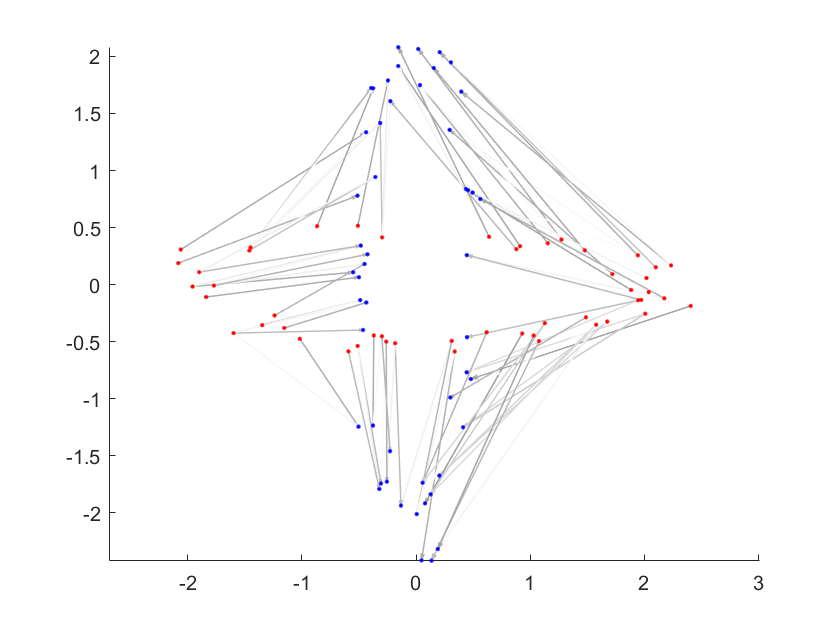
\includegraphics[width=12cm]{final/ellipse1.png}
\caption{An Ellipse Example with sample size $n=50$. The darker the line, the greater the $\pi_{i, j}$.}
\label{ellipse}
\end{figure}

\subsubsection{Caffarelli's Example}
This example, mentioned in \cite{multiscale}, consists of two uniform samples on $[-1, 1]^2$ of size $n$. Then any point outside the unit circle are then discarded. The source and target data sample is split along the x-Axis at 0 and shifted by -2 and +2, respectively. Note that the true number of points may be less than $n$. When $n$ is large, about $\frac{\pi}{4}n$ points are preserved. For ease of notation, we still assume there are $n$ points. The corresponding parameter for the standard form of LP is as follows. $m = n$, $\mu_i=1, \nu_i=1(i=1, ..., n)$ and $C_{i, j}=\|x_i-y_j\|_2$, which is the Euclidean distance between two points $x_i$ and $y_j$. Figure \ref{caff} gives an example.
\begin{figure}[h]
\centering
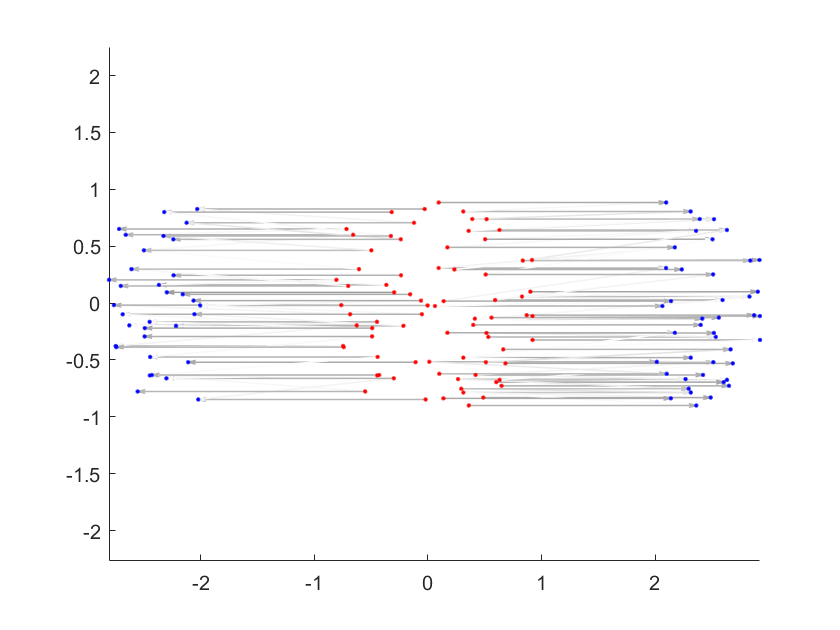
\includegraphics[width=12cm]{final/caff1.png}
\caption{An Caffarelli's Example with sample size $n=50$. The darker the line, the greater the $\pi_{i, j}$.}
\label{caff}
\end{figure}

\subsubsection{Gaussian Mixture Model}
Suppose $p_\mu$ and $p_\nu$ are the probability density function of two different Gaussian mixture models and $N$ is the number of discrete points. In this example, $\mu$ and $\nu$ are the normalized discrete distribution of Gaussian mixture models, which satisfy
$$
\mu_i=\frac{p_\mu(\frac{i-1}{N-1})}{\sum_{i=1}^Np_\mu(\frac{i-1}{N-1})}, \quad \nu_j=\frac{p_\nu(\frac{j-1}{N-1})}{\sum_{j=1}^Np_\nu(\frac{j-1}{N-1})}
$$
And $C_{i,j}=|i-j|$. 

\subsection{Different methods on Mosek and Gurobi}
`prim', `dual', `int' represent primal simplex, dual simplex and interior point method respectively. `(M)' means Mosek, `(G)' means Gurobi. For each method, we record the time and the number of iteration it takes and evaluate their performance. We examine the accuracy of the solution $\pi$ by the value of the objective function ('objval') 
$$
\sum_{i=1}^m\sum_{j=1}^nC_{i,j}\pi_{i,j}
$$
and the violation of the constraints ('vltcst') 
$$
\sum_{i=1}^m|\mu_i - \sum_{j=1}^{n}\pi_{i, j}| + \sum_{j=1}^n|\nu_j-\sum_{i=1}^m\pi_{i, j}|$$
In the table, we only give the exact value of `objval' for prim(M). In `objval' of other methods, we give its relative difference to prim(M). Namely, if `objval' for prim(M) is $f_1$ and `objval' for prim(G) is $f_2$, in `objval' of prim(G), we give $\frac{f_1-f_2}{f_1}$. 

\subsubsection{Randomly generated data}
For simplicity, we only consider the case when $m=n$. We take $m=128,256,512,1024$.  

\begin{table}[h]
\caption{Perfomance of mosek and gurobi on randomly generated data}
\label{RGD_mg}
\centering
\begin{tabular} {|c|c|c|c|c|c|c|c|} 
\hline
\multicolumn{2}{|c|}{method}&prim(M)&dual(M)&int(M)&prim(G)&dual(G)&int(G)\\\hline
\multirow{4}*{\makecell{$m=128$\\$n=128$}} 
&time(s)& 0.05 & 0.04 & 0.08 & 0.07 & 0.03 & 0.08 \\\cline{2-8}
&iter& 1488 & 220 & 13 & 3101 & 204 & 13 \\\cline{2-8}
&objval& 1.36e+00 & -6.08e-06 & -6.08e-06 & -6.08e-06 & -6.08e-06 & -6.08e-06 \\\cline{2-8}
&vltcst& 1.11e-05 & 5.55e-17 & 1.14e-10 & 4.94e-17 & 4.94e-17 & 4.94e-17 \\\hline
\multirow{4}*{\makecell{$m=256$\\$n=256$}} 
&time(s)& 0.21 & 0.18 & 0.33 & 0.20 & 0.14 & 0.30 \\\cline{2-8}
&iter& 4708 & 480 & 13 & 9252 & 437 & 15 \\\cline{2-8}
&objval& 1.63e+00 & -1.90e-05 & -1.90e-05 & -1.90e-05 & -1.90e-05 & -1.90e-05 \\\cline{2-8}
&vltcst& 3.62e-05 & 4.99e-17 & 1.05e-10 & 7.81e-18 & 6.51e-18 & 7.81e-18 \\\hline
\multirow{4}*{\makecell{$m=512$\\$n=512$}} 
&time(s)& 0.95 & 1.38 & 1.99 & 1.17 & 0.63 & 2.06 \\\cline{2-8}
&iter& 11742 & 472 & 15 & 32211 & 2266 & 19 \\\cline{2-8}
&objval& 1.57e+00 & -4.76e-05 & -4.76e-05 & -4.76e-05 & -4.76e-05 & -4.76e-05 \\\cline{2-8}
&vltcst& 9.14e-05 & 1.73e-16 & 1.44e-12 & 7.42e-17 & 7.42e-17 & 7.42e-17 \\\hline

\multirow{4}*{\makecell{$m=1024$\\$n=1024$}} 
&time(s)& 5.39 & 11.95 & 11.37 & 6.28 & 3.13 & 12.32 \\\cline{2-8}
&iter& 28914 & 2299 & 18 & 108153 & 6020 & 23 \\\cline{2-8}
&objval& 1.94e+00 & -1.21e-04 & -1.21e-04 & -1.21e-04 & -1.21e-04 & -1.21e-04 \\\cline{2-8}
&vltcst& 2.31e-04 & 3.51e-16 & 2.85e-11 & 4.68e-17 & 4.66e-17 & 4.68e-17 \\\hline

\end{tabular}
\end{table}

From Table \ref{RGD_mg}, we can see on Mosek, dual simplex method and interior point method take much more time than primal simplex does, especially when $m, n$ are large. But on Gurobi, dual simplex method is the fastest method and the time primal simplex method takes is close to the time interior point takes. Interior point method takes much smaller number of iterations than  We can observe that compared to other methods, primal simplex method on Mosek gets the largest value of objective function and the largest value of the violation of constraints. On Mosek, dual simplex methods achieves the lowest value of `vltcst', which partly explains why it takes the longest time. On Gurobi, the solution from all methods satisfies constraints perfectly.

\subsubsection{DOTmark}
We then test the performance of Mosek and Gurobi on DOTmark \cite{DOTmark}. We number the classes of DOTmark with the order of alphabet in the following way.
\begin{table}[!htp]
\centering
\begin{tabular}{|c|c|c|c|c|}
\hline
CauchyDensity&ClassicImages&GRFmoderate&GRFrough&GRFsmooth\\\hline
1&2&3&4&5\\\hline
LogGRF&LogitGRF&MicroscopyImages&Shapes&WhiteNoise\\\hline
6&7&8&9&10\\\hline
\end{tabular}
\end{table}

We test on pictures with resolution $32\times32$. 
\begin{table}[htbp]
\caption{Perfomance of mosek and gurobi on DOTmark}
\label{DOTmark_mg}
\centering
\begin{tabular} {|c|c|c|c|c|c|c|c|} 
\hline
Class No.&method&prim(M)&dual(M)&int(M)&prim(G)&dual(G)&int(G)\\\hline
\multirow{4}*{1} 
&time(s)& 5.53 & 52.84 & 11.34 & 5.17 & 6.49 & 10.51 \\\cline{2-8}
&iter& 23489 & 13515 & 16 & 74691 & 58692 & 17 \\\cline{2-8}
&objval& 1.75e+01 & -1.54e-05 & -1.53e-05 & -1.53e-05 & -1.54e-05 & -1.53e-05 \\\cline{2-8}
&vltcst& 2.34e-05 & 3.28e-16 & 5.53e-12 & 1.48e-17 & 2.11e-17 & 2.53e-17 \\\hline
\multirow{4}*{2} 
&time(s)& 5.76 & 26.44 & 11.39 & 4.95 & 4.57 & 11.12 \\\cline{2-8}
&iter& 22163 & 7634 & 16 & 85161 & 24036 & 17 \\\cline{2-8}
&objval& 6.27e+00 & 6.43e-07 & 6.43e-07 & 6.43e-07 & 6.43e-07 & 6.43e-07 \\\cline{2-8}
&vltcst& 2.67e-05 & 2.37e-16 & 1.92e-11 & 8.57e-18 & 1.01e-17 & 8.81e-18 \\\hline
\multirow{4}*{3} 
&time(s)& 5.12 & 26.71 & 11.12 & 4.76 & 3.79 & 10.43 \\\cline{2-8}
&iter& 21240 & 7395 & 16 & 81109 & 16455 & 15 \\\cline{2-8}
&objval& 4.07e+00 & 2.50e-05 & 2.50e-05 & 2.50e-05 & 2.50e-05 & 2.50e-05 \\\cline{2-8}
&vltcst& 2.89e-05 & 3.56e-17 & 6.41e-14 & 1.11e-17 & 8.73e-18 & 1.12e-17 \\\hline
\multirow{4}*{4} 
&time(s)& 5.09 & 19.64 & 11.11 & 5.10 & 3.01 & 10.73 \\\cline{2-8}
&iter& 22063 & 4493 & 17 & 88412 & 7513 & 16 \\\cline{2-8}
&objval& 1.48e+00 & 1.69e-05 & 1.69e-05 & 1.69e-05 & 1.69e-05 & 1.69e-05 \\\cline{2-8}
&vltcst& 2.77e-05 & 9.29e-17 & 9.24e-11 & 1.56e-17 & 1.38e-17 & 1.59e-17 \\\hline
\multirow{4}*{5} 
&time(s)& 5.17 & 37.87 & 10.59 & 4.62 & 6.29 & 10.41 \\\cline{2-8}
&iter& 21509 & 11384 & 14 & 85058 & 43743 & 15 \\\cline{2-8}
&objval& 2.14e+01 & -3.71e-06 & -3.71e-06 & -3.71e-06 & -3.79e-06 & -3.71e-06 \\\cline{2-8}
&vltcst& 2.98e-05 & 1.16e-16 & 3.72e-10 & 1.04e-17 & 7.75e-18 & 1.03e-17 \\\hline
\multirow{4}*{6} 
&time(s)& 5.70 & 27.97 & 10.92 & 4.88 & 5.69 & 10.63 \\\cline{2-8}
&iter& 22635 & 8991 & 14 & 82331 & 40023 & 15 \\\cline{2-8}
&objval& 1.92e+01 & 5.65e-06 & 5.65e-06 & 5.65e-06 & 5.65e-06 & 5.65e-06 \\\cline{2-8}
&vltcst& 2.49e-05 & 2.97e-16 & 2.03e-11 & 2.20e-17 & 2.21e-17 & 1.95e-17 \\\hline
\multirow{4}*{7} 
&time(s)& 5.32 & 28.00 & 10.98 & 5.07 & 6.10 & 10.14 \\\cline{2-8}
&iter& 22695 & 9302 & 14 & 85918 & 36763 & 15 \\\cline{2-8}
&objval& 1.69e+01 & 2.69e-06 & 2.69e-06 & 2.69e-06 & 2.69e-06 & 2.69e-06 \\\cline{2-8}
&vltcst& 2.57e-05 & 2.29e-16 & 1.57e-09 & 1.22e-17 & 1.35e-17 & 1.66e-17 \\\hline
\multirow{4}*{8} 
&time(s)& 3.40 & 6.98 & 5.49 & 4.11 & 3.17 & 4.81 \\\cline{2-8}
&iter& 15322 & 4493 & 17 & 77555 & 14763 & 17 \\\cline{2-8}
&objval& 1.09e+01 & -1.45e-05 & -1.45e-05 & -1.45e-05 & -1.45e-05 & -1.45e-05 \\\cline{2-8}
&vltcst& 1.56e-05 & 2.19e-16 & 7.59e-12 & 4.33e-17 & 4.89e-17 & 5.28e-17 \\\hline
\multirow{4}*{9} 
&time(s)& 2.62 & 7.51 & 3.78 & 2.12 & 2.21 & 2.28 \\\cline{2-8}
&iter& 12983 & 5418 & 9 & 4616 & 2075 & 10 \\\cline{2-8}
&objval& 2.44e+01 & 1.69e-05 & 1.70e-05 & 1.69e-05 & 1.69e-05 & 1.69e-05 \\\cline{2-8}
&vltcst& 2.04e-05 & 7.50e-17 & 1.87e-08 & 2.08e-17 & 2.08e-17 & 2.08e-17 \\\hline
\multirow{4}*{10} 
&time(s)& 5.41 & 13.07 & 10.51 & 5.08 & 2.60 & 11.20 \\\cline{2-8}
&iter& 23237 & 2545 & 14 & 92953 & 4390 & 17 \\\cline{2-8}
&objval& 7.09e-01 & 3.08e-05 & 3.12e-05 & 3.08e-05 & 3.08e-05 & 3.08e-05 \\\cline{2-8}
&vltcst& 2.60e-05 & 3.13e-16 & 1.60e-09 & 2.42e-17 & 2.17e-17 & 2.59e-17 \\\hline
\end{tabular}
\end{table}

From Table \ref{DOTmark_mg}, we observe that dual simplex method on Mosek takes much longer time than other methods. The cpu-time of primal simplex method on Mosek and primal simplex method and dual simplex method on Gurobi are close. On Mosek and Gurobi, the iteration number vary with different classes of DOTmark. Compared to other methods, primal simplex method on Mosek gets the largest `vltcst' and the largest `vltcst'. On Mosek, dual simplex methods achieves the smallest `vltcst'. On Gurobi , the solution $\pi$ from all methods satisfies the constraints perfectly.

\subsubsection{Ellipse Example \& Caffarelli's Example}
Similar to randomly generated data, we only consider the case when $m=n$. We take $m=128,256,512,1024$.  
\begin{table}[htbp]
\caption{Perfomance of mosek and gurobi on Ellipse Example}
\label{ellipse_mg}
\centering
\begin{tabular} {|c|c|c|c|c|c|c|c|} 
\hline
\multicolumn{2}{|c|}{method}&prim(M)&dual(M)&int(M)&prim(G)&dual(G)&int(G)\\\hline
\multirow{4}*{\makecell{$m=128$\\$n=128$}} 
&time(s)& 0.10 & 0.13 & 0.08 & 0.05 & 0.14 & 0.08 \\\cline{2-8}
&iter& 1675 & 1497 & 12 & 2965 & 1302 & 16 \\\cline{2-8}
&objval& 2.57e+00 & -6.86e-06 & -6.86e-06 & -6.86e-06 & -6.86e-06 & -6.86e-06 \\\cline{2-8}
&vltcst& 1.33e-05 & 1.04e-17 & 7.49e-10 & 5.20e-18 & 6.07e-18 & 5.20e-18 \\\hline

\multirow{4}*{\makecell{$m=256$\\$n=256$}} 
&time(s)& 0.18 & 0.86 & 0.40 & 0.19 & 1.38 & 0.32 \\\cline{2-8}
&iter& 4112 & 3968 & 16 & 8966 & 3664 & 16 \\\cline{2-8}
&objval& 2.48e+00 & -1.77e-05 & -1.77e-05 & -1.77e-05 & -1.77e-05 & -1.77e-05 \\\cline{2-8}
&vltcst& 3.48e-05 & 2.13e-17 & 1.11e-10 & 1.39e-17 & 1.47e-17 & 1.47e-17 \\\hline

\multirow{4}*{\makecell{$m=512$\\$n=512$}} 
&time(s)& 0.86 & 9.26 & 2.16 & 0.92 & 2.05 & 1.95 \\\cline{2-8}
&iter& 9528 & 12791 & 19 & 25763 & 42487 & 17 \\\cline{2-8}
&objval& 2.28e+00 & -4.32e-05 & -4.32e-05 & -4.32e-05 & -4.32e-05 & -4.32e-05 \\\cline{2-8}
&vltcst& 8.55e-05 & 1.00e-16 & 3.09e-12 & 6.20e-17 & 6.14e-17 & 6.18e-17 \\\hline

\multirow{4}*{\makecell{$m=1024$\\$n=1024$}} 
&time(s)& 5.25 & 96.98 & 12.30 & 4.97 & 11.51 & 11.05 \\\cline{2-8}
&iter& 21756 & 33591 & 20 & 79738 & 152520 & 19 \\\cline{2-8}
&objval& 2.25e+00 & -9.83e-05 & -9.83e-05 & -9.83e-05 & -9.83e-05 & -9.83e-05 \\\cline{2-8}
&vltcst& 1.96e-04 & 9.45e-17 & 4.96e-13 & 2.63e-17 & 2.69e-17 & 2.65e-17 \\\hline
\end{tabular}
\end{table}
\begin{table}[htbp]
\caption{Perfomance of mosek and gurobi on Caffarelli's Example}
\label{caff_mg}
\centering
\begin{tabular} {|c|c|c|c|c|c|c|c|} 
\hline
\multicolumn{2}{|c|}{method}&prim(M)&dual(M)&int(M)&prim(G)&dual(G)&int(G)\\\hline
\multirow{4}*{\makecell{$m=128$\\$n=128$}} 
&time(s)& 0.04 & 0.06 & 0.06 & 0.05 & 0.05 & 0.06 \\\cline{2-8}
&iter& 1370 & 795 & 14 & 2061 & 820 & 15 \\\cline{2-8}
&objval& 4.00e+00 & -5.58e-06 & -5.58e-06 & -5.58e-06 & -5.58e-06 & -5.58e-06 \\\cline{2-8}
&vltcst& 1.09e-05 & 3.12e-17 & 6.02e-12 & 3.12e-17 & 3.12e-17 & 3.12e-17 \\\hline

\multirow{4}*{\makecell{$m=256$\\$n=256$}} 
&time(s)& 0.11 & 0.26 & 0.21 & 0.10 & 0.35 & 0.19 \\\cline{2-8}
&iter& 3016 & 1996 & 15 & 6373 & 2157 & 15 \\\cline{2-8}
&objval& 4.00e+00 & -1.34e-05 & -1.34e-05 & -1.34e-05 & -1.34e-05 & -1.34e-05 \\\cline{2-8}
&vltcst& 2.60e-05 & 6.77e-17 & 5.81e-14 & 6.42e-17 & 6.42e-17 & 6.42e-17 \\\hline

\multirow{4}*{\makecell{$m=512$\\$n=512$}} 
&time(s)& 0.45 & 2.33 & 1.11 & 0.52 & 0.88 & 0.96 \\\cline{2-8}
&iter& 7536 & 5588 & 18 & 21406 & 19906 & 17 \\\cline{2-8}
&objval& 4.01e+00 & -3.40e-05 & -3.40e-05 & -3.40e-05 & -3.40e-05 & -3.40e-05 \\\cline{2-8}
&vltcst& 6.70e-05 & 7.11e-17 & 1.13e-12 & 4.08e-17 & 4.08e-17 & 4.08e-17 \\\hline

\multirow{4}*{\makecell{$m=1024$\\$n=1024$}} 
&time(s)& 2.27 & 24.16 & 5.87 & 2.53 & 4.70 & 4.82 \\\cline{2-8}
&iter& 17237 & 15464 &19 & 62128 & 68342 & 18 \\\cline{2-8}
&objval& 4.00e+00 & -7.75e-05 & -7.75e-05 & -7.75e-05 & -7.75e-05 & -7.75e-05 \\\cline{2-8}
&vltcst& 1.54e-04 & 9.50e-17 & 4.83e-12 & 4.29e-17 & 4.29e-17 & 4.29e-17 \\\hline
\end{tabular}
\end{table}

Different from the results on randomly generated data, Table \ref{ellipse_mg} shows that on Ellipse Example, dual simplex method takes much longer time and more iterations than primal simplex method, no matter on Mosek or on Gurobi. Similar to Ellipse Example, Table \ref{caff_mg} shows that dual simplex method takes much longer time than the primal simplex method, no matter on Mosek or on Gurobi. The iteration number of primal simplex method and dual simplex method are close. Similarly, compared to other methods, primal simplex method on Mosek gets the largest `vltcst' and the largest `vltcst'. On Mosek, dual simplex methods achieves the smallest `vltcst'. On Gurobi , the solution $\pi$ from all methods satisfies the constraints perfectly.

\subsection{First order methods}
`prim(M)' means primal method of Mosek. `ADMM-p' means ADMM primal method \ref{alg:ADMM}. `ADMM-d' means ADMM dual method \ref{alg:ADMM-dual}. `ADMM-s' means another ADMM splitting method for primal problem \ref{alg:ADMM-split}. BADMM means Bregman ADMM \ref{alg:BADMM}.
\subsubsection{Art of Tuning Parameters}
The success of ADMM always lies in an appropriate choice of the coefficient $t$ in the quadratic term of the augmented Lagrangian function. Thanks to the normalization of constraints, i.e., letting $\sum_{i=1}^m\mu_i = \sum_{j=1}^n\nu_j = 1$, the tuning of parameters is relatively easier. Intuitively, the value of $t$ should be dependent on the problem size, $m$ and $n$, and the objective coefficients $C$. In our implementation, for primal problem, we let $t$ to be proportional to $(m+n)\bar C$, where $\bar C$ is the mean of the coefficient matrix $C$ ($\frac{1}{mn}\sum_{i, j}C_{i, j}$). For dual problem, we set $t$ to be inversely proportional to $(m+n)\bar C$. For the Bregman ADMM, we set $t$ to be proportional to $\bar C$. The detailed proportion will be clear in the following. Empirically, we found that such strategy performs well in our experiments.

\subsubsection{Randomly Generated Data}
\begin{table}[htbp]
\caption{Perfomance of first order methods on randomly generated data}
\label{RGD_fo}
\centering
\begin{tabular} {|c|c|c|c|c|c|c|} 
\hline
\multicolumn{2}{|c|}{method}&prim(M)&ADMM-p&ADMM-d&ADMM-s&BADMM\\\hline
\multirow{4}*{\makecell{$m=128$\\$n=128$}} 
&time(s) & 0.10 & 2.44 & 1.01 & 3.50 & 1.91 \\\cline{2-7}
&iter & 1488 & 13405 & 5534 & 3466 & 7640 \\\cline{2-7}
&objval & 1.36e+00 & -3.29e-06 & 1.32e-05 & 4.10e-06 & 3.26e-05 \\\cline{2-7}
&vltcst & 1.11e-05 & 5.00e-07 & 1.99e-04 & 8.29e-08 & 1.95e-05 \\\hline
\multirow{4}*{\makecell{$m=256$\\$n=256$}} 
&time(s) & 0.20 & 9.00 & 5.92 & 40.22 & 9.75 \\\cline{2-7}
&iter & 4708 & 17525 & 12309 & 11542 & 9986 \\\cline{2-7}
&objval & 1.63e+00 & -9.92e-06 & -6.07e-06 & -8.76e-06 & 5.88e-05 \\\cline{2-7}
&vltcst & 3.62e-05 & 5.00e-07 & 2.00e-04 & 9.51e-08 & 1.94e-05 \\\hline

\multirow{4}*{\makecell{$m=512$\\$n=512$}} 
&time(s) & 0.97 & 47.85 & 41.07 & 187.57 & 76.40 \\\cline{2-7}
&iter & 11742 & 14719 & 15561 & 11863 & 12732 \\\cline{2-7}
&objval & 1.57e+00 & -3.16e-05 & -3.88e-05 & -4.46e-05 & 8.87e-06 \\\cline{2-7}
&vltcst & 9.14e-05 & 5.00e-07 & 2.00e-04 & 9.89e-08 & 4.35e-05 \\\hline

\multirow{4}*{\makecell{$m=1024$\\$n=1024$}} 
&time(s) & 5.68 & 205.60 & 232.08 & 902.93 & 432.45 \\\cline{2-7}
&iter & 28914 & 14403 & 20000 & 13163 & 15564 \\\cline{2-7}
&objval & 1.94e+00 & -1.10e-04 & -1.18e-04 & -1.18e-04 & -9.02e-05 \\\cline{2-7}
&vltcst & 2.31e-04 & 5.00e-07 & 2.76e-04 & 9.94e-08 & 6.34e-05 \\\hline
\end{tabular}
\end{table}
In Table \ref{RGD_fo}, we present the numerical results on random generated data. 
Detailed tuning parameters is listed in Table \ref{param_rgd_fo}.
\begin{table}[h]
\centering
\caption{Tuned Parameters: Random Generated Data}
\label{param_rgd_fo}
\begin{tabular}{|c|c|c|}
\hline 
Solver & $t$ & Stopping Rule \\
\hline
ADMM-p & $5(m+n)\bar C$ & $\text{`vltcst'}\leqslant$ 5e-07 or $\text{`iter'}\geqslant$ 2e+04 \\\hline
ADMM-d & $1/(8(m+n)\bar C)$ & $\text{`vltcst'}\leqslant$ 2e-04 or $\text{`iter'}\geqslant$ 2e+04 \\\hline
ADMM-s & $2(m+n)\bar C$ & $\text{`vltcst'}\leqslant$ 1e-07 or $\text{`iter'}\geqslant$ 2e+04 \\\hline
BADMM & $10\bar C$ & $\|\pi-\tilde\pi\|_1\leqslant$ 1e-06 or $\text{`iter'}\geqslant$ 2e+04 \\
\hline
\end{tabular}
\end{table}

In this setting, both `ADMM-p' and `ADMM-s' achieves relatively better results. They both satisfy the constraints quite well and achieve lower objective value. `ADMM-p' spends moderate time in all problems because all computation has closed form. `ADMM-s' performs quite well in `objval' and `vltcst', especially when the problem size is larger. However, such accuracy is at the cost of much longer time. In fact, from our observation, much of the time by `ADMM-s' is spent on the projection on the simplex(constraints). There exists more efficient algorithms for projection, but since time is limited, we do not implement them. The projection is quite essential in `ADMM-s' because it imposes $\pi$ to satisfy constraints, and this may explain why the constraints are easy to satisfy within tolerance.

It's worth noting that `ADMM-d' has weakness in satisfying constraints. This is because in Section 2.1.2 we regard the ``dual of dual'' as an approximation of initial variables, which is numerically unstable. In our experiments, we found that `ADMM-d' converges faster at the beginning to the optimal value, but then continuously vibrates around optimal value for a long time. `BADMM' appears to perform worse than other three algorithms. The selection of $t$ is inconsistent with other ADMM due to the property of KL divergence. If $t$ is selected to be too big, then the exponential term in \ref{badmm_pipit_upd} may be so close to 1 that leads to bad precision. Furthermore, in our experiments, we found that when we increase $t$, `BADMM' indeed has slightly better performance in `vltcst' but deteriorates rapidly in `objval'. Our parameter is a balance between the two targets.

\subsubsection{DOTmark}
Some detailed tuning parameters is listed in Table \ref{param_DOTmark_fo}.
\begin{table}[htbp]
\centering
\caption{Tuned Parameters: DOTmark}
\label{param_DOTmark_fo}
\begin{tabular}{|c|c|c|}
\hline 
Solver & $t$ & Stopping Rule \\
\hline
ADMM-p & $5(m+n)\bar C$ & $\text{`vltcst'}\leqslant$ 5e-07 or $\text{`iter'}\geqslant$ 2e+04 \\\hline
ADMM-d & $1/(8(m+n)\bar C)$ & $\text{`vltcst'}\leqslant$ 2e-04 or $\text{`iter'}\geqslant$ 2e+04 \\\hline
ADMM-s & $2(m+n)\bar C$ & $\text{`vltcst'}\leqslant$ 4e-07 or $\text{`iter'}\geqslant$ 2e+04 \\\hline
BADMM & $10\bar C$ & $\|\pi-\tilde\pi\|_1\leqslant$ 4e-06 or $\text{`iter'}\geqslant$ 2e+04 \\
\hline
\end{tabular}
\end{table}

\begin{table}[htbp]
\caption{Perfomance of first order methods on DOTmark}
\label{DOTmark_fo}
\centering
\begin{tabular} {|c|c|c|c|c|c|c|} 
\hline
\multicolumn{2}{|c|}{method}&prim(M)&ADMM-p&ADMM-d&ADMM-s&BADMM\\\hline
\multirow{4}*{1} 
&time(s) & 5.44 & 128.59 & 174.96 & 620.48 & 615.58 \\\cline{2-7}
&iter & 23489 & 8974 & 15247 & 10958 & 20000 \\\cline{2-7}
&objval & 1.75e+01 & 1.83e-03 & 2.49e-03 & 9.05e-04 & -4.35e-03 \\\cline{2-7}
&vltcst & 2.34e-05 & 4.99e-07 & 2.00e-04 & 3.94e-07 & 8.22e-04 \\\hline
\multirow{4}*{2} 
&time(s) & 5.52 & 128.18 & 154.83 & 448.70 & 607.74 \\\cline{2-7}
&iter & 22163 & 8942 & 13427 & 7746 & 20000 \\\cline{2-7}
&objval & 6.27e+00 & 2.51e-03 & 9.22e-05 & 1.94e-04 & -1.03e-03 \\\cline{2-7}
&vltcst & 2.67e-05 & 5.00e-07 & 2.00e-04 & 3.87e-07 & 2.47e-04 \\\hline
\multirow{4}*{3} 
&time(s) & 5.23 & 141.67 & 181.92 & 474.67 &607.68 \\\cline{2-7}
&iter & 21240 & 9940 & 15782 & 8142 & 20000 \\\cline{2-7}
&objval & 4.07e+00 & -2.90e-03 & -6.66e-04 & 2.84e-04 & 7.53e-05 \\\cline{2-7}
&vltcst & 2.89e-05 & 4.99e-07 & 2.00e-04 & 3.91e-07 & 1.60e-04 \\\hline
\multirow{4}*{4} 
&time(s) & 5.56 & 133.39 & 156.39 & 525.16 & 610.47 \\\cline{2-7}
&iter & 20163 & 9316 & 13560 & 8970 & 20000 \\\cline{2-7}
&objval & 1.48e+00 & 2.67e-03 & 3.33e-04 & 2.74e-04 & 3.77e-03 \\\cline{2-7}
&vltcst & 2.77e-05 & 5.00e-07 & 2.00e-04 & 3.88e-07 & 6.34e-05 \\\hline
\multirow{4}*{5} 
&time(s) & 5.29 & 143.51 & 182.07 & 468.54 & 615.51 \\\cline{2-7}
&iter & 21509 & 10035 & 15795 & 8183 & 20000 \\\cline{2-7}
&objval & 2.14e+01 & -1.62e-03 & -3.89e-04 & -3.46e-06 & -1.56e-03 \\\cline{2-7}
&vltcst & 2.98e-05 & 5.00e-07 & 2.00e-04 & 3.22e-07 & 3.87e-04 \\\hline
\multirow{4}*{6} 
&time(s) & 5.50 & 124.36 & 163.82 & 420.16 & 616.91 \\\cline{2-7}
&iter & 22635 & 8688 & 14282 & 7290 & 20000 \\\cline{2-7}
&objval & 1.92e+01 & 1.19e-03 & 3.89e-04 & 3.67e-04 & -8.27e-04 \\\cline{2-7}
&vltcst & 2.49e-05 & 4.99e-07 & 2.00e-04 & 3.40e-07 & 3.38e-04 \\\hline
\multirow{4}*{7} 
&time(s) & 5.51 & 139.22 & 165.99 & 511.25 & 614.00 \\\cline{2-7}
&iter & 22695 & 9726 & 14478 & 8894 & 20000 \\\cline{2-7}
&objval & 1.69e+01 & -7.46e-04 & 2.79e-04 & 4.85e-05 & -1.67e-03 \\\cline{2-7}
&vltcst & 2.57e-05 & 4.99e-07 & 2.00e-04 & 3.85e-07 & 3.54e-04 \\\hline
\multirow{4}*{8} 
&time(s) & 3.60 & 120.51 & 157.94 & 399.11 & 619.88 \\\cline{2-7}              
&iter & 15322 & 8401 & 13672 & 6812 & 20000 \\\cline{2-7}                          
&objval & 1.09e+01 & 1.89e-03 & 1.44e-03 & 1.46e-03 & 7.32e-05 \\\cline{2-7}        
&vltcst & 1.56e-05 & 5.00e-07 & 2.00e-04 & 3.73e-07 & 7.87e-05 \\\hline  
\multirow{4}*{9} 
&time(s) & 2.68 & 93.18 & 121.59 & 115.47 & 207.71 \\\cline{2-7}               
&iter & 12983 & 6514 & 10589 & 2000 & 20000 \\\cline{2-7}                          
&objval & 2.44e+01 & -2.36e-04 & 1.09e-04 & 9.24e-04 & 7.93e-06 \\\cline{2-7}       
&vltcst & 2.04e-05 & 4.97e-07 & 2.00e-04 & 3.69e-07 & 3.73e-05 \\\hline 
\multirow{4}*{10} 
&time(s) & 5.49 & 106.63 & 155.21 & 516.34 & 346.73 \\\cline{2-7}               
&iter & 23237 & 7428 & 13515 & 8776 & 2508 \\\cline{2-7}                           
&objval & 7.09e-01 & 1.75e-03 & 1.31e-03 & 4.63e-04 & 2.87e-02 \\\cline{2-7}   
&vltcst & 2.60e-05 & 5.00e-07 & 2.00e-04 & 3.81e-07 & 6.65e-05 \\\hline
\end{tabular}
\end{table}
Table \ref{DOTmark_fo} presents the numerical results on DOTmark.

As to constraints, all methods perform similar to that in the setting of random generated data, since our stopping rule is built on `vltcst' or the norm of difference between $\pi$ and $\tilde\pi$. 

As to objective value, the three traditional ADMM methods are not stable on `objval' and tend to achieve higher value than Mosek. This may be because of the different structure between random generated data and DOTmark. `BADMM' tends to achieve lower objective value. However, the results are not stable and the constraints are not satisfied well.

As to iteration numbers and time spent, surprisingly, `ADMM-p' and `ADMM-s' need much less iterations than others. This phenomenon implies that we could tighten our stopping rule by decreasing the thresholds. Due to the time limit, further experiments could be conducted in the future.

\subsubsection{Ellipse Example \& Caffarelli's Example}
The detailed parameters is listed in Table \ref{param_ellcaff_fo}. 
\begin{table}[htbp]
\centering
\caption{Tuning Parameters: Ellipse \& Caffarelli}
\label{param_ellcaff_fo}
\begin{tabular}{|c|c|c|}
\hline 
Solver & $t$ & Stopping Rule \\
\hline
ADMM-p & $5(m+n)\bar C$ & $\text{`vltcst'}\leqslant$ 5e-07 or $\text{`iter'}\geqslant$ 2e+04 \\\hline
ADMM-d & $1/(8(m+n)\bar C)$ & $\text{`vltcst'}\leqslant$ 2e-04 or $\text{`iter'}\geqslant$ 2e+04 \\\hline
ADMM-s & $2(m+n)\bar C$ & $\text{`vltcst'}\leqslant$ 2e-07 or $\text{`iter'}\geqslant$ 2e+04 \\\hline
BADMM & $10\bar C$ & $\|\pi-\tilde\pi\|_1\leqslant$ 4e-06 or $\text{`iter'}\geqslant$ 2e+04 \\
\hline
\end{tabular}
\end{table}

\begin{table}[htbp]
\caption{Perfomance of first order methods on Ellipse Example}
\label{ellipse_fo}
\centering
\begin{tabular} {|c|c|c|c|c|c|c|} 
\hline
\multicolumn{2}{|c|}{method}&prim(M)&ADMM-p&ADMM-d&ADMM-s&BADMM\\\hline
\multirow{4}*{\makecell{$m=128$\\$n=128$}} 
&time(s) & 0.10 & 2.62 & 1.73 & 9.34 & 3.37 \\\cline{2-7}
&iter & 1675 & 14454 & 9692 & 9515 & 10830 \\\cline{2-7}
&objval & 2.57e+00 & 3.22e-05 & 1.07e-04 & 4.49e-05 & 4.68e-04 \\\cline{2-7}
&vltcst & 1.33e-05 & 4.99e-07 & 9.99e-05 & 2.00e-07 & 1.95e-05 \\\hline

\multirow{4}*{\makecell{$m=256$\\$n=256$}} 
&time(s) & 0.19 & 4.32 & 4.51 & 34.93 & 30.86 \\\cline{2-7}
&iter & 4112 & 8287 & 9186 & 10075 & 18006 \\\cline{2-7}
&objval & 2.48e+00 & 1.02e-04 & 1.75e-04 & 5.46e-05 & 3.30e-04 \\\cline{2-7}
&vltcst & 3.48e-05 & 4.99e-07 & 9.96e-05 & 1.89e-07 & 6.35e-05 \\\hline

\multirow{4}*{\makecell{$m=512$\\$n=512$}} 
&time(s) & 0.88 & 22.48 & 29.94 & 265.18 & 155.61 \\\cline{2-7}
&iter & 9528 & 6863 & 11434 & 16927 & 20000 \\\cline{2-7}
&objval & 2.28e+00 & 1.39e-04 & 1.27e-04 & 1.30e-05 & -3.60e-05 \\\cline{2-7}
&vltcst & 8.55e-05 & 4.99e-07 & 9.98e-05 & 1.97e-07 & 7.12e-04 \\\hline

\multirow{4}*{\makecell{$m=1024$\\$n=1024$}} 
&time(s) & 5.29 & 60.14 & 229.84 & 1161.15 & 616.73 \\\cline{2-7}
&iter & 21756 & 4178 & 20000 & 16527 & 20000 \\\cline{2-7}
&objval & 2.25e+00 & 1.58e-04 & 4.24e-06 & -4.07e-05 & -3.55e-03 \\\cline{2-7}
&vltcst & 1.96e-04 & 5.00e-07 & 1.14e-04 & 1.99e-07 & 6.16e-03 \\\hline
\end{tabular}
\end{table}
\begin{table}[htbp]
\caption{Perfomance of first order methods on Caffarelli's Example}
\label{caff_fo}
\centering
\begin{tabular} {|c|c|c|c|c|c|c|} 
\hline
\multicolumn{2}{|c|}{method}&prim(M)&ADMM-p&ADMM-d&ADMM-s&BADMM\\\hline
\multirow{4}*{\makecell{$m=128$\\$n=128$}} 
&time(s) & 0.04 & 1.30 & 0.90 & 3.61 & 2.12 \\\cline{2-7}
&iter & 1370 & 8605 & 5910 & 5587 & 9588 \\\cline{2-7}
&objval & 4.00e+00 & 6.75e-05 & 2.54e-04 & 9.05e-05 & 4.19e-04 \\\cline{2-7}
&vltcst & 1.09e-05 & 4.99e-07 & 9.91e-05 & 1.61e-07 & 1.74e-05 \\\hline

\multirow{4}*{\makecell{$m=256$\\$n=256$}} 
&time(s) & 0.10 & 3.31 & 3.26 & 23.06 & 14.54 \\\cline{2-7}
&iter & 3016 & 9177 & 9444 & 10788 & 15936 \\\cline{2-7}
&objval & 4.00e+00 & 6.99e-05 & 1.67e-04 & 3.30e-05 & 2.38e-04 \\\cline{2-7}
&vltcst & 2.60e-05 & 5.00e-07 & 9.98e-05 & 1.95e-07 & 2.58e-05 \\\hline

\multirow{4}*{\makecell{$m=512$\\$n=512$}} 
&time(s) & 0.47 & 12.88 & 16.67 & 114.61 & 80.05 \\\cline{2-7}
&iter & 7536 & 6612 & 10983 & 12057 & 20000 \\\cline{2-7}
&objval & 4.01e+00 & 1.48e-04 & 1.51e-04 & 3.32e-05 & 2.43e-04 \\\cline{2-7}
&vltcst & 6.70e-05 & 4.99e-07 & 1.00e-04 & 1.96e-07 & 1.13e-04 \\\hline

\multirow{4}*{\makecell{$m=1024$\\$n=1024$}} 
&time(s) & 2.33 & 47.56 & 123.05 & 841.48 & 328.21 \\\cline{2-7}
&iter & 17237 & 5052 & 16104 & 20000 & 20000 \\\cline{2-7}
&objval & 4.00e+00 & 1.84e-04 & 6.40e-05 & -3.31e-05 & -4.43e-05 \\\cline{2-7}
&vltcst & 1.54e-04 & 4.99e-07 & 1.00e-04 & 6.56e-07 & 1.49e-03 \\\hline
\end{tabular}
\end{table}

Table \ref{ellipse_fo} and \ref{caff_fo} presents numerical results for Ellipse Example and Caffarelli's Example, respectively.

The constraints are generally satisfied before we stop iterations. The solution from `BADMM' does not satisfy the constraints very well. However, the optimal value is not within our expectation. The vibration of objective values around optimal values are observed in the three traditional ADMM methods. Among these algorithms, `ADMM-s' performs relatively better on `iter', `objval', and `vltcst', though it takes more time in each iteration. Nevertheless, `objval' of `BADMM' is relatively low.

\subsection{Algorithms for entropic regularized OT}
`sinkhorn' represents the Sinkhorn's algorithm with numerical stability and continuation strategy \ref{alg:sansc}. `ADMM' means the algorithm described in \ref{alg:ADMM-ER}. Addition to `time', `iter', `objval' and `vltcst', we use `entval' to denote the objective value with extropy regularization term. The values in `objval' are, same as before, compared to `prim(M)'.

The parameters and stopping criterions of our algorithms are given in Table \ref{param_er}. In 'sinkhorn', we apply continuation strategy. If the coefficient of the regularized term is $\epsilon$, we select $10^i\epsilon(i=4, 3, 2, 1, 0)$ as the sequence and run 4000 iterations in optimizing every subproblem.

\begin{table}[htbp]
\centering
\caption{Tuned Parameters: algorithms for entropic regularized OT}
\label{param_er}
\begin{tabular}{|c|c|c|}
\hline 
method & $t$ & Stopping Rule \\
\hline
ADMM & $5(m+n)\bar C$ & $\text{`vltcst'}\leqslant$ 1e-07 or $\text{`iter'}\geqslant$ 2e+04 \\\hline
sinkhorn & / & $\text{`iter'}\geqslant$ 2e+04 \\
\hline
\end{tabular}
\end{table}

\subsubsection{Gaussian Mixture Model: The effect of continuation strategy}

We consider to test Sinkhorn's algorithm with numerical stability on Gaussian mixture model and test the effect of continuation strategy. We first take $N=128$ as a first exmaple. Figure \ref{gmm3} gives the probability density function of two Gaussian mixture models.
\begin{figure}[htbp]
\centering
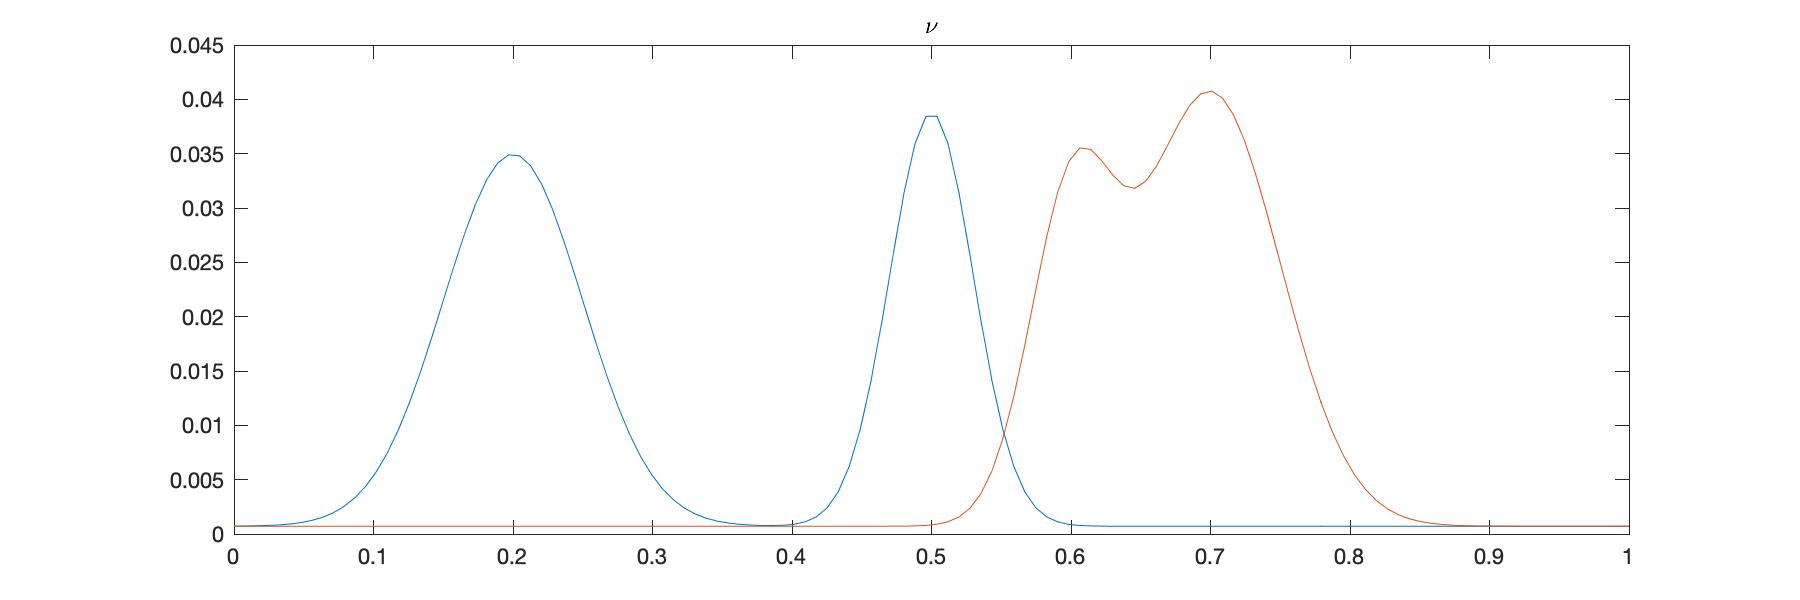
\includegraphics[width=12cm]{final/gmm3.jpg}
\caption{The probability distribution function of two Gaussian mixture models $G_1$ and $G_2$. $G_1$ (blue one) has mean $[0.2,0.5]$, variance $[0.05^2, 0.03^2]$ and component proportion $[0.6, 0.4]$; $G_2$ (red one) has mean $[0.6,0.7]$, variance $[0.03^2, 0.05^2]$ and component proportion $[0.3, 0.7]$. }
\label{gmm3}
\end{figure}

We then take $\epsilon=10^{-2},10^{-3},10^{-4},10^{-5}$. If we use the vanilla Sinkhorn's algorithm \ref{alg:sa} for $\epsilon=10^{-4},10^{-5}$, $K^{\epsilon}$ would be a zero matrix. For Sinkhorn's algorithm with numerical stability \ref{alg:sans}, we take the maximum iteration number to be $10,100,1000,4000$ respectively. For Sinkhorn's algorithm with numerical stability and continuation strategy \ref{alg:sansc}, we take $\alpha=0.1$, $\epsilon_0=\epsilon\times 10^5$ and the maximum iteration number to be $2,20,200,800$ respectively. 

\begin{figure}[!htb]
\centering
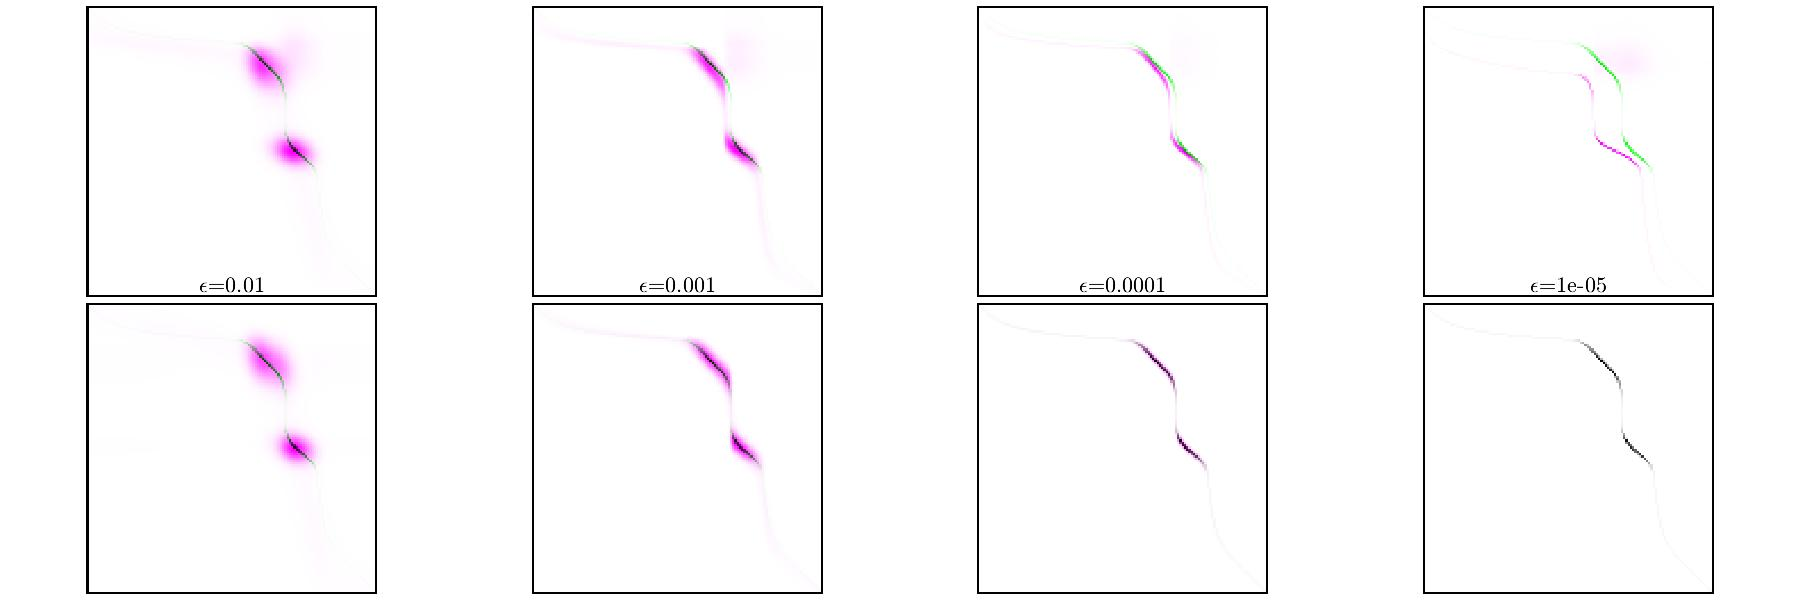
\includegraphics[width=12cm]{final/gmm4.jpg}
	\caption{Impact of $\epsilon$ on the coupling between two gaussian mixture models \ref{gmm1}. From left to right, $\epsilon=10^{-2},10^{-3},10^{-4},10^{-5}$. The upper row is without continuation strategy and the lower row is with continuatation strategy. The purple one is the solution to the entropic regularized LP. The green one is the solution to the original LP.}
\label{gmm4}
\end{figure}

From Figure \ref{gmm4}, we can find that with same iteration number, Sinkhorn's algorithm with numerical stability and continuation strategy converges faster than the one only with numerical stability. This shows that with proper choice of the parameter of continuation, we can achieve acceleration in Sinkhorn's algorithm with continuation strategy.

We then perform a comprehensive numerical experiment on Gaussian mixture model. Detailed parameters and the stopping criterions are listed in Table \ref{param_er}. 

\begin{table}[htbp]
\caption{Perfomance of algorithms for entropic regularization of OT on Gaussian mixture model}
\label{gmm_er}
\centering
\begin{tabular} {|c|c|c|c|c|c|c|c|} 
\hline
\multicolumn{2}{|c|}{ }&\multicolumn{2}{c|}{$\epsilon=10^{-2}$}
&\multicolumn{2}{c|}{$\epsilon=10^{-4}$}
&\multicolumn{2}{c|}{$\epsilon=10^{-6}$}\\
\hline
\multicolumn{2}{|c|}{method}&sinkhorn&ADMM&sinkhorn&ADMM&sinkhorn&ADMM\\\hline
\multirow{4}*{\makecell{$m=128$\\$n=128$}} 
& time(s) & 10.39 & 0.23 & 9.52 & 0.85 & 7.92 & 6.19 \\\cline{2-8}              
& iter & 20000 & 647 & 20000 & 2398 & 20000 & 20000 \\\cline{2-8}               
& objval & 7.25e-02 & 7.24e-02 & 6.77e-04 & 2.19e-03 & 1.76e-04 & 2.32e-04 \\\cline{2-8}                                                                        
& entval & -2.50e-02 & -2.50e-02 & 5.20e-02 & 5.20e-02 & 5.26e-02 & 5.26e-02 \\\cline{2-8}                                                                      
& vltcst & 1.27e-12 & 9.93e-08 & 6.15e-14 & 9.96e-08 & 5.14e-12 & 3.83e-07 \\\hline

\multirow{4}*{\makecell{$m=256$\\$n=256$}} 
& time(s) & 34.53 & 1.34 & 31.96 & 1.90 & 25.48 & 18.53 \\\cline{2-8}           
& iter & 20000 & 1213 & 20000 & 1782 & 20000 & 18203 \\\cline{2-8}              
& objval & 7.27e-02 & 7.26e-02 & 8.55e-04 & 1.85e-03 & 4.94e-04 & 2.74e-04 \\\cline{2-8}                                                                        
& entval & -3.89e-02 & -3.89e-02 & 5.19e-02 & 5.19e-02 & 5.26e-02 & 5.26e-02 \\\cline{2-8}
& vltcst & 1.37e-12 & 9.96e-08 & 1.17e-13 & 9.91e-08 & 3.83e-12 & 9.98e-08 \\\hline

\multirow{4}*{\makecell{$m=512$\\$n=512$}} 
& time(s) & 140.15 & 12.56 & 130.25 & 11.82 & 104.53 & 56.03 \\\cline{2-8}     
& iter & 20000 & 2228 & 20000 & 2100 & 20000 & 9939 \\\cline{2-8}              
& objval & 7.27e-02 & 7.26e-02 & 8.95e-04 & 1.44e-03 & 2.07e-04 & 3.22e-04 \\\cline{2-8}
& entval & -5.28e-02 & -5.28e-02 & 5.17e-02 & 5.17e-02 & 5.26e-02 & 5.26e-02 \\\cline{2-8}
& vltcst & 1.42e-12 & 9.99e-08 & 8.56e-14 & 9.99e-08 & 1.58e-12 & 9.97e-08 \\\hline

\multirow{4}*{\makecell{$m=1024$\\$n=1024$}} 
& time(s) & 692.47 & 99.56 & 658.32 & 86.61 & 557.13 & 144.90 \\\cline{2-8}
& iter & 20000 & 4034 & 20000 & 3523 & 20000 & 5896 \\\cline{2-8}
& objval & 7.27e-02 & 7.24e-02 & 8.79e-04 & 7.20e-04 & 1.84e-04 & 4.07e-04 \\\cline{2-8}
& entval & -6.67e-02 & -6.67e-02 & 5.16e-02 & 5.16e-02 & 5.26e-02 & 5.26e-02 \\\cline{2-8}
& vltcst & 1.29e-12 & 9.99e-08 & 1.30e-13 & 1.00e-07 & 1.49e-12 & 1.00e-07 \\\hline

\end{tabular}
\end{table}
Table \ref{gmm_er} gives the comprehensive numerical results for Gaussian Mixture Model. The setting is same as Figure \ref{gmm1}, except that we test examples for different problem sizes, i.e., we let $N=128, 256, 512, 1024$, respectively. We observe that, in most cases, although `sinkhorn' takes much longer time and more iterations than `ADMM', `sinkhorn' outperforms `ADMM' in both `objval' and `vltcst'. 

\subsubsection{Randomly generated data}
The parameters and the stopping criterions are listed in Table \ref{param_er}. Table \ref{RGD_er} presents numerical results on random generated data. 

\begin{table}[htbp]
\caption{Perfomance of algorithms for entropic regularization of OT on randomly generated data}
\label{RGD_er}
\centering
\begin{tabular} {|c|c|c|c|c|c|c|c|} 
\hline
\multicolumn{2}{|c|}{ }&\multicolumn{2}{c|}{$\epsilon=10^{-2}$}
&\multicolumn{2}{c|}{$\epsilon=10^{-4}$}
&\multicolumn{2}{c|}{$\epsilon=10^{-6}$}\\
\hline
\multicolumn{2}{|c|}{method}&sinkhorn&ADMM&sinkhorn&ADMM&sinkhorn&ADMM\\\hline
\multirow{4}*{\makecell{$m=128$\\$n=128$}} 
& time(s) & 10.06 & 0.82 & 8.36 & 6.16 & 6.84 & 6.21 \\\cline{2-8}             
& iter & 20000 & 2223 & 20000 & 20000 & 20000 & 20000 \\\cline{2-8}            
& objval & 2.40e-04 & 3.18e-04 & 1.23e-03 & -6.35e-06 & 2.54e-03 & -8.73e-06 \\\cline{2-8}                                                                     
& entval & 1.30e+00 & 1.30e+00 & 1.36e+00 & 1.36e+00 & 1.36e+00 & 1.36e+00 \\\cline{2-8}                                                                       
& vltcst & 6.48e-15 & 9.99e-08 & 6.60e-13 & 2.22e-07 & 9.86e-11 & 4.72e-07 \\\hline

\multirow{4}*{\makecell{$m=256$\\$n=256$}} 
& time(s) & 32.66 & 3.23 & 26.86 & 19.88 & 20.49 & 20.46 \\\cline{2-8}         
& iter & 20000 & 3072 & 20000 & 20000 & 20000 & 20000 \\\cline{2-8}            
& objval & 3.16e-04 & 3.49e-04 & 2.36e-03 & -9.92e-06 & 4.52e-03 & -1.24e-05 \\\cline{2-8}                                                                     
& entval & 1.56e+00 & 1.56e+00 & 1.63e+00 & 1.62e+00 & 1.63e+00 & 1.63e+00 \\\cline{2-8}
& vltcst & 2.98e-15 & 9.99e-08 & 7.04e-13 & 5.62e-07 & 1.28e-10 & 6.90e-07 \\\hline

\multirow{4}*{\makecell{$m=512$\\$n=512$}} 
& time(s) & 134.57 & 17.43 & 108.35 & 111.25 & 83.80 & 111.31 \\\cline{2-8}    
& iter & 20000 & 3045 & 20000 & 20000 & 20000 & 20000 \\\cline{2-8}            
& objval & 3.48e-04 & 3.76e-04 & 1.55e-03 & -4.66e-05 & 3.43e-03 & -4.69e-05 \\\cline{2-8}
& entval & 1.49e+00 & 1.49e+00 & 1.57e+00 & 1.57e+00 & 1.57e+00 & 1.57e+00 \\\cline{2-8}
& vltcst & 9.34e-15 & 9.98e-08 & 7.69e-13 & 2.18e-07 & 8.42e-11 & 3.08e-07 \\\hline

\multirow{4}*{\makecell{$m=1024$\\$n=1024$}} 
& time(s) & 692.35 & 99.61 & 568.16 & 497.03 & 472.21 & 495.21 \\\cline{2-8}   
& iter & 20000 & 4040 & 20000 & 20000 & 20000 & 20000 \\\cline{2-8}            
& objval & 2.11e-04 & 2.04e-04 & 1.93e-03 & -1.15e-04 & 3.54e-03 & -1.23e-04 \\\cline{2-8}
& entval & 1.85e+00 & 1.85e+00 & 1.94e+00 & 1.93e+00 & 1.94e+00 & 1.94e+00 \\\cline{2-8}
& vltcst & 1.63e-14 & 9.97e-08 & 1.22e-12 & 2.18e-07 & 1.06e-10 & 2.99e-07 \\\hline

\end{tabular}
\end{table}

We find that the `objval' and `vltcst' of `sinkhorn' is getting worse with the decrease of $\epsilon$. This can be explained by the computation complexity of Sinkhorn's algorithm. As shown in Section 3.2, the $\tau$-approximate solution of the unregularized OT problem takes $O(n^2\log(n)\tau^{-3})$ operations where $\epsilon=\tau/\log(n)$. This means that if we decrease the $\epsilon$ by $0.1$, theoretically we would need $10^3$ times iteration to get a precise solution. Although our improvements of Sinkhorn's algorithm makes it adapt to small $\epsilon$, but the computation is costly. If we want to use Sinkhorn's algorithm to get an approximation solution of the orignial problem \ref{lp}, we should pay attention to choose an appropriate $\epsilon$. 

On the contrary, `ADMM' appears robustness in satisfying constraints within acceptable iteration number. `vltcst' of all test samples are below 1e-06, though it's not comparable to `sinkhorn'. `objval' of ADMM appears to be gradually lower than `prim(M)' when $\epsilon$ decreases. It's worth noting that in `ADMM' we do not apply continuation strategy. In fact, we observe that with the carefully selected $t$, `ADMM' converges quite fast to the optimal value at the beginning, whatever $\epsilon$ is, although vibration is unavoidable in the latter steps. Of course, for $\epsilon$ not large and small or moderate problem sizes, `sinkhorn' performs better than `ADMM'.


\subsubsection{DOTmark}
Detailed parameters are listed in \ref{param_er}. (The stopping rule for `ADMM' changes to $\text{`vltcst'}\leqslant$ 1e-07 or $\text{`iter'}\geqslant$ 2e+04.) Table \ref{DOTmark_er1} and \ref{DOTmark_er2} present numerical results on DOTmark.
\begin{table}[htbp]
\caption{Perfomance of algorithms for entropic regularization of OT on DOTmark Part1}
\label{DOTmark_er1}
\centering
\begin{tabular} {|c|c|c|c|c|c|c|c|} 
\hline
\multicolumn{2}{|c|}{ }&\multicolumn{2}{c|}{$\epsilon=10^{-2}$}
&\multicolumn{2}{c|}{$\epsilon=10^{-4}$}
&\multicolumn{2}{c|}{$\epsilon=10^{-6}$}\\
\hline
Class No.&method &sinkhorn&ADMM&sinkhorn&ADMM&sinkhorn&ADMM\\\hline
\multirow{4}*{1} 
& time(s) & 593.54 & 335.53 & 502.26 & 369.18 & 440.68 & 371.82 \\\cline{
2-8}                                                                            
& iter & 20000 & 13674 & 20000 & 15058 & 20000 & 15062 \\\cline{2-8}        
& objval& 2.01e-02 & 8.30e-04 & 3.36e-02 & 6.52e-04 & 2.11e+00 & 7.27e-04 \\\cline{2-8}                                                             
& entval & 1.78e+01 & 1.74e+01 & 1.81e+01 & 1.75e+01 & 5.44e+01 & 1.75e+01 \\\cline{2-8}                                                             
& vltcst & 2.87e-13 & 2.00e-07 & 2.38e-11 & 2.00e-07 & 6.03e-10 & 2.00e-07 \\\hline 

\multirow{4}*{2} 
& time(s) & 610.36 & 264.70 & 499.11 & 318.66 & 445.02 & 318.45 \\\cline{2-8}                                                                            
& iter & 20000 & 10740 & 20000 & 13021 & 20000 & 13021 \\\cline{2-8}        
& objval & 4.60e-02 & -1.17e-03 & 7.43e-02 & 4.09e-04 & 5.86e+00 & 4.29e-04 \\\cline{2-8}                                                            
& entval & 6.47e+00 & 6.18e+00 & 6.74e+00 & 6.27e+00 & 4.30e+01 & 6.07e+00 \\\cline{2-8}                                                             
& vltcst & 1.46e-13 & 2.00e-07 & 1.69e-11 & 2.00e-07 & 3.80e-10 & 2.00e-07 \\\hline

\multirow{4}*{3} 
& time(s)& 591.98 & 299.63 & 499.19 & 361.14 & 442.04 & 361.33 \\\cline{2-8}
& iter & 20000 & 12206 & 20000 & 14672 & 20000 & 14668 \\\cline{2-8}
& objval & 8.12e-02 & 3.74e-04 & 2.46e-01 & -1.14e-03 & 6.45e+00 & -1.11e-03 \\\cline{2-8}
& entval & 4.32e+00 & 3.99e+00 & 5.07e+00 & 4.07e+00 & 3.03e+01 & 4.07e+00 \\\cline{2-8}
& vltcst & 1.52e-13 & 2.00e-07 & 9.59e-12 & 2.00e-07 & 2.85e-10 & 2.00e-07 \\\hline

\multirow{4}*{4}
& time(s) & 591.00 & 268.63 & 499.50 & 330.66 & 441.70 & 331.92 \\\cline{2-8}
& iter & 20000 & 10923 & 20000 & 13433 & 20000 & 13467 \\\cline{2-8}
& objval & 2.18e-01 & -1.26e-03 & 4.58e-01 & -5.81e-04 & 9.30e+00 & -5.05e-04 \\\cline{2-8}
& entval  & 1.71e+00 & 1.39e+00 & 2.15e+00 & 1.47e+00 & 1.52e+01 & 1.48e+00 \\\cline{2-8}
& vltcst & 1.17e-13 & 2.00e-07 & 6.78e-12 & 2.00e-07 & 2.35e-10 & 2.00e-07 \\\hline

\multirow{4}*{5}
& time(s) & 589.61 & 295.34 & 499.33 & 368.54 & 442.19 & 368.14 \\\cline{2-8}
& iter & 20000 & 12018 & 20000 & 15052 & 20000 & 15047 \\\cline{2-8}
& objval &  8.86e-03 & 8.71e-04 & 3.55e-02 & 9.91e-04 & 2.46e+00 & 9.9
4e-04 \\\cline{2-8}
& entval & 2.15e+01 & 2.13e+01 & 2.22e+01 & 2.14e+01 & 7.41e+01 & 2.14e+01 \\\cline{2-8}
& vltcst & 1.97e-13 & 2.00e-07 & 3.58e-11 & 2.00e-07 & 5.87e-10 & 2.00e-07 \\\hline

\multirow{4}*{6}
& time(s) & 590.35 & 253.97 & 498.56 & 326.70 & 441.70 & 327.49 \\\cline{2-8}
& iter & 20000 & 10339 & 20000 & 13362 & 20000 & 13385 \\\cline{2-8}
& objval & 1.10e-02 & 2.37e-04 & 3.88e-02 & -3.33e-04 & 2.17e+00 & -3.35e-04 \\\cline{2-8}
& entval & 1.93e+01 & 1.91e+01 & 1.99e+01 & 1.92e+01 & 6.09e+01 & 1.92e+01 \\\cline{2-8}
& vltcst & 3.53e-13 & 2.00e-07 & 3.24e-11 & 2.00e-07 & 8.49e-10 & 2.00e-07 \\\hline

\multirow{4}*{7} 
& time(s) & 590.12 & 296.02 & 499.00 & 339.12 & 441.04 & 339.56 \\\cline{2-8}
& iter & 20000 & 12054 & 20000 & 13862 & 20000 & 13877 \\\cline{2-8}
& objval  & 1.60e-02 & 9.12e-04 & 4.17e-02 & -4.18e-04 & 2.82e+00 & -4.48e-04 \\\cline{2-8}
& entval & 1.71e+01 & 1.69e+01 & 1.76e+01 & 1.69e+01 & 6.48e+01 & 1.69e+01 \\\cline{2-8}
& vltcst & 3.62e-13 & 2.00e-07 & 3.62e-11 & 2.00e-07 & 6.20e-10 & 2.00e-07 \\\hline

\end{tabular}
\end{table}
\begin{table}[htbp]
\caption{Perfomance of algorithms for entropic regularization of OT on DOTmark Part2}
\label{DOTmark_er2}
\centering
\begin{tabular} {|c|c|c|c|c|c|c|c|} 
\hline
\multicolumn{2}{|c|}{ }&\multicolumn{2}{c|}{$\epsilon=10^{-2}$}
&\multicolumn{2}{c|}{$\epsilon=10^{-4}$}
&\multicolumn{2}{c|}{$\epsilon=10^{-6}$}\\
\hline
Class No.&method &sinkhorn&ADMM&sinkhorn&ADMM&sinkhorn&ADMM\\\hline

\multirow{4}*{8} 
& time(s) & 604.68 & 273.63 & 502.38 & 374.75 & 441.42 & 374.83 \\\cline{2-8}                                                                            
& iter & 20000 & 11185 & 20000 & 15318 & 20000 & 15323 \\\cline{2-8}        
& objval & 3.30e-02 & 6.25e-04 & 4.21e-02 & -1.95e-04 & 2.01e+00 & -2.27e-04 \\\cline{2-8}                                                           
& entval & 1.12e+01 & 1.08e+01 & 1.13e+01 & 1.09e+01 & 3.27e+01 & 1.09e+01 \\\cline{2-8}                                                             
& vltcst & 5.46e-13 & 2.00e-07 & 1.72e-11 & 2.00e-07 & 8.71e-10 & 2.00e-07 \\\hline

\multirow{4}*{9} 
& time(s) & 603.00 & 249.23 & 501.40 & 299.38 & 439.78 & 264.61 \\\cline{2-8}
& iter & 20000 & 10177 & 20000 & 12241 & 20000 & 10814 \\\cline{2-8}
& objval & 1.69e-05 & 4.17e-05 & 1.69e-05 & -7.33e-05 & 7.96e-01 & 9.68e-05 \\\cline{2-8}
& entval  & 2.43e+01 & 2.43e+01 & 2.44e+01 & 2.44e+01 & 4.38e+01 & 2.24e+01 \\\cline{2-8}
& vltcst   & 6.59e-13 & 1.98e-07 & 2.73e-11 & 1.99e-07 & 5.95e-10 & 1.99e-07 \\\hline

\multirow{4}*{10}
& time(s) & 590.49 & 237.95 & 500.10 & 281.92 & 441.94 & 282.65 \\\cline{2-8}
& iter & 20000 & 9693 & 20000 & 11524 & 20000 & 11549 \\\cline{2-8}
& objval & 4.20e-01 & 1.98e-03 & 1.25e+00 & -1.02e-03 & 7.78e+00 & -1.21e-04 \\\cline{2-8}
& entval & 9.22e-01 & 6.25e-01 & 1.60e+00 & 7.08e-01 & 6.23e+00 & 7.09e-01 \\\cline{2-8}
& vltcst & 2.17e-13 & 2.00e-07 & 2.16e-12 & 2.00e-07 & 1.18e-10 & 2.00e-07 \\\hline

\end{tabular}
\end{table}

Same as before, `objval' and `vltcst' of `sinkhorn' is getting worse with the decrease of $\epsilon$. All of the results are within 1e-09 in `vltcst', but `objval' deteriorate rapidly when $\epsilon$ decreases. This can be again explained by the computation complexity of Sinkhorn's algorithm. 

'ADMM' can achieve relatively lower objective value on average, and need moderate iterations before `vltcst' arrives at a threshold. The performance is similar to random generated data setting with larger problem sizes. We should note that due to the different problem structures, it seems difficult sometimes for `ADMM' to outperform `prim(M)'.

\subsubsection{Ellipse Example \& Caffarelli's Example}
\begin{table}[htbp]
\caption{Perfomance of algorithms for entropic regularization of OT on Ellipse Example}
\label{ellipse_er}
\centering
\begin{tabular} {|c|c|c|c|c|c|c|c|} 
\hline
\multicolumn{2}{|c|}{ }&\multicolumn{2}{c|}{$\epsilon=10^{-2}$}
&\multicolumn{2}{c|}{$\epsilon=10^{-4}$}
&\multicolumn{2}{c|}{$\epsilon=10^{-6}$}\\
\hline
\multicolumn{2}{|c|}{method}&sinkhorn&ADMM&sinkhorn&ADMM&sinkhorn&ADMM\\\hline
\multirow{4}*{\makecell{$m=128$\\$n=128$}} 
& time(s) & 10.04 & 0.36 & 8.91 & 6.23 & 7.18 & 6.21 \\\cline{2-8}              
& iter & 20000 & 984 & 20000 & 20000 & 20000 & 20000 \\\cline{2-8}              
& objval & 1.77e-03 & 2.24e-03 & 5.91e-04 & 1.58e-05 & 4.66e-03 & 7.81e-06 \\\cline{2-8}                                                                        
& entval & 2.50e+00 & 2.50e+00 & 2.57e+00 & 2.57e+00 & 2.58e+00 & 2.57e+00 \\\cline{2-8}                                                                        
& vltcst & 1.90e-14 & 9.95e-08 & 3.11e-13 & 3.85e-07 & 9.03e-11 & 5.63e-07 \\\hline  

\multirow{4}*{\makecell{$m=256$\\$n=256$}} 
& time(s) & 33.01 & 0.81 & 29.70 & 19.50 & 22.52 & 20.14 \\\cline{2-8}          
& iter & 20000 & 705 & 20000 & 19370 & 20000 & 20000 \\\cline{2-8}              
& objval & 2.37e-03 & 2.72e-03 & 3.32e-04 & 2.71e-05 & 1.58e-03 & 1.97e-05 \\\cline{2-8}                                                                        
& entval & 2.40e+00 & 2.40e+00 & 2.48e+00 & 2.48e+00 & 2.49e+00 & 2.48e+00 \\\cline{2-8}
& vltcst & 1.42e-14 & 9.91e-08 & 9.55e-13 & 9.97e-08 & 9.77e-11 & 2.43e-07 \\\hline

\multirow{4}*{\makecell{$m=512$\\$n=512$}} 
& time(s) & 134.58 & 3.57 & 119.84 & 91.35 & 91.55 & 112.25 \\\cline{2-8}
& iter & 20000 & 637 & 20000 & 16276 & 20000 & 20000 \\\cline{2-8}
& objval & 3.06e-03 & 3.27e-03 & 2.80e-04 & 3.83e-05 & 1.51e-03 & 1.62e-05 \\\cline{2-8}
& entval & 2.19e+00 & 2.19e+00 & 2.28e+00 & 2.28e+00 & 2.28e+00 & 2.28e+00 \\\cline{2-8}
& vltcst & 1.37e-14 & 9.92e-08 & 1.19e-12 & 9.99e-08 & 1.42e-10 & 2.36e-07 \\\hline

\multirow{4}*{\makecell{$m=1024$\\$n=1024$}} 
& time(s) & 677.72 & 15.72 & 625.73 & 386.85 & 514.66 & 491.65 \\\cline{2-8}
& iter & 20000 & 641 & 20000 & 15739 & 20000 & 20000 \\\cline{2-8}
& objval & 3.40e-03 & 3.48e-03 & 7.94e-05 & -1.92e-05 & 1.61e-03 & -3.87e-05 \\\cline{2-8}
& entval & 2.15e+00 & 2.15e+00 & 2.25e+00 & 2.25e+00 & 2.26e+00 & 2.25e+00 \\\cline{2-8}
& vltcst & 1.37e-14 & 1.00e-07 & 7.50e-13 & 9.99e-08 & 1.30e-10 & 1.46e-07 \\\hline

\end{tabular}
\end{table}
\begin{table}[htbp]
\caption{Perfomance of algorithms for entropic regularization of OT on Caffarelli's Example}
\label{caff_er}
\centering
\begin{tabular} {|c|c|c|c|c|c|c|c|} 
\hline
\multicolumn{2}{|c|}{ }&\multicolumn{2}{c|}{$\epsilon=10^{-2}$}
&\multicolumn{2}{c|}{$\epsilon=10^{-4}$}
&\multicolumn{2}{c|}{$\epsilon=10^{-6}$}\\
\hline
\multicolumn{2}{|c|}{method}&sinkhorn&ADMM&sinkhorn&ADMM&sinkhorn&ADMM\\\hline
\multirow{4}*{\makecell{$m=128$\\$n=128$}} 
& time(s) & 7.61 & 0.50 & 6.76 & 4.64 & 5.58 & 4.66 \\\cline{2-8}               
& iter & 20000 & 1777 & 20000 & 20000 & 20000 & 20000 \\\cline{2-8}             
& objval & 1.03e-03 & 1.45e-03 & 5.04e-04 & 9.71e-06 & 4.01e-04 & 6.89e-06 \\\cline{2-8}                                                                        
& entval & 3.93e+00 & 3.93e+00 & 4.00e+00 & 4.00e+00 & 4.00e+00 & 4.00e+00 \\\cline{2-8}                                                                        
& vltcst & 9.94e-15 & 9.98e-08 & 2.81e-12 & 1.63e-07 & 2.12e-10 & 2.94e-07 \\\hline

\multirow{4}*{\makecell{$m=256$\\$n=256$}} 
& time(s) & 21.63 & 0.84 & 19.52 & 13.12 & 15.29 & 13.09 \\\cline{2-8}          
& iter & 20000 & 1154 & 20000 & 20000 & 20000 & 20000 \\\cline{2-8}             
& objval & 1.40e-03 & 1.90e-03 & 4.87e-04 & 1.32e-05 & 8.98e-04 & 1.18e-05 \\\cline{2-8}                                                                        
& entval & 3.93e+00 & 3.93e+00 & 4.00e+00 & 4.00e+00 & 4.01e+00 & 4.00e+00 \\\cline{2-8}
& vltcst & 1.18e-14 & 9.95e-08 & 1.47e-12 & 1.67e-07 & 1.88e-10 & 2.37e-07 \\\hline

\multirow{4}*{\makecell{$m=512$\\$n=512$}} 
& time(s) & 83.29 & 2.20 & 74.29 & 68.36 & 55.97 & 68.35 \\\cline{2-8}
& iter & 20000 & 644 & 20000 & 20000 & 20000 & 20000 \\\cline{2-8}
& objval & 1.73e-03 & 2.25e-03 & 1.40e-03 & 1.18e-05 & 1.78e-03 & 9.34e-06 \\\cline{2-8}
& entval & 3.92e+00 & 3.92e+00 & 4.01e+00 & 4.00e+00 & 4.01e+00 & 4.01e+00 \\\cline{2-8}
& vltcst & 1.44e-14 & 9.97e-08 & 1.21e-12 & 1.28e-07 & 1.70e-10 & 1.98e-07 \\\hline

\multirow{4}*{\makecell{$m=1024$\\$n=1024$}} 
& time(s) & 428.49 & 11.31 & 390.39 & 256.87 & 320.54 & 321.15 \\\cline{2-8}
& iter & 20000 & 704 & 20000 & 16004 & 20000 & 20000 \\\cline{2-8}
& objval & 2.01e-03 & 2.19e-03 & 6.65e-04 & 7.60e-06 & 1.32e-03 & -1.46e-05 \\\cline{2-8}
& entval & 3.90e+00 & 3.90e+00 & 4.00e+00 & 4.00e+00 & 4.00e+00 & 4.00e+00 \\\cline{2-8}
& vltcst & 1.67e-14 & 9.86e-08 & 1.83e-12 & 9.99e-08 & 2.17e-10 & 1.48e-07 \\\hline

\end{tabular}
\end{table}
Table \ref{param_er} lists the detailed parameters.Table \ref{ellipse_er} and Table \ref{caff_er} present numerical results for Ellipse Example and Caffarelli's Example, respectively. Through our previous experiments, we observe that with the decrease of $\epsilon$, `ADMM' does not require so much increase of computational complexity as `sinkhorn'. This can be explained by the limit when $\epsilon\to0$. When $\epsilon\to0$, `ADMM' reduce to ADMM for the primal problem \ref{lp}. But with $\epsilon\to0$, we have shown in Section 3.3.1 that `sinkhorn' will diverge due to the loss of strong convexity. And with the decrease of $\epsilon$, the strong convexity of problem \ref{equ:kl} decreases. This also explains why `sinkhorn' requires such enormous iterations to find the optimal solution. In summary, we shall use `sinkhorn' to solve the entropic regularization of OT \ref{equ:kl} with moderate $\epsilon$. With large $\epsilon$, we shall use the original Sinkhorn's algorithm \ref{alg:sa} because it is faster in computation. `ADMM' seems to be suitable to arbitrary small $\epsilon$. 


\section{Conclusion}
\label{sec:5}
Our work for OT (Optimal Transport) ends up here, but new ideas for improvement and continuous passion for research will never fade. We now give a brief summary for what we have done and give some outlooks.

We first implemented several first-order methods, mainly `ADMM's. Generally, they do not perform very well if compared to state-of-art algorithm packages such as Gurobi. However, the violation of constraints and optimality of objective values are within our tolerance. From our experiments, directly solving primal problems are much better than solving dual ones. Needless to say, it has been considered that first-order methods such as `ADMM' are not suitable for large-scale OT problems. But we observe that first-order methods could also achieve relatively satisfying results, if we choose smart splitting schemes and tuning parameters.

We then choose Entropy Regularization as our main topic. Sinkhorn is a theoretically and practically elegant algorithm. However, numerical stability and convergence speed cause difficulty in optimizing the regularized problem, especially when the coefficient of regularized term $\epsilon$ is small. We adopt a technique to improve the stability and the continuation strategy to boost convergence. Great improvement has been observed, but deterioration of performance when $\epsilon$ is very small still exists. It's worth mentioning that ADMM shows moderate results on Entropy Regularization.

Now we provide some future outlooks. For first order methods, we hope to implement the interior point algorithm to deal with constraints satisfaction. In addition, second-order algorithms like Newton methods and semi-smooth Newton methods can be tested out. Also, as is mentioned before, projection on a simplex in first order methods can be further simplified to reduce iteration time. Furthermore, though we have testified that our choice of parameters achieve good results, theoretical properties remained to be studied.

For Sinkhorn's method, we hope to continue on refining the numerical stability and boosting convergence. A simple method is to combine Sinkhorn with other methods such as ADMM. Additionally, if time has permitted, we might want to try implementing the algorithm in C++ in order to accelerate processing. 

For numerical experiments, we hope to test on the whole DOTmark to have a more precise investigation on the accuracy and efficiency of all these algorithms. 

Transportation problem is the basis for many high level applications. However, solving the problem is still tough even with numerous proposed methods. Of course, we hope that we can find more efficient methods, both in time and space. This will be left for future research.

\section*{Acknowledgement}
We would like to thank Zeyu Jia a lot for providing his server to let us run our numerical experiments. 

The division of our work is listed below. Yifei Wang is responsible for the writing and coding of Bregman ADMM (Section 2.3), Sinkhorn's algorithm and related methods (Section 3.1-3.3); the framework of coding and the conducting of most of the numerical experiments in Section 4. Feng Zhu is responsible for the writing and coding of ADMMs and related methods (Section 2.1-2.2, Section 3.4, Appendix); the writing of most of the experiment reports in Section 4. 

\printbibliography
\begin{appendix}
\section*{Appendix: Splitting method with penalty functions}

To impose more attention on constraints, we propose the following splitting method with penalty functions.

Let $F(\pi)$ and $G(\pi)$ be defined in the following way,
\begin{eqt}
& F(\pi) = \sum_{i, j}C_{i,j}\pi_{i,j} + \frac{t}{2}\left(\sum_{i}(\mu_i-\sum_{j}\pi_{i,j})^2 + \sum_{j}(\nu_j-\sum_{i}\pi_{i,j})^2\right) \\
& G(\pi) = 
\left\{
\begin{matrix}
0, \indent &\pi_{i, j}\geqslant0,\ \forall i, j\\
+\infty, \indent &\text{else}
\end{matrix}
\right.
\end{eqt}
Now let the problem be
\begin{eqt}
\min_\pi \ F(\pi) + G(\pi)
\end{eqt}
It's easy to obtain
\begin{eqt}
\text{prox}_{\frac{1}{w}G}(\pi) = \max\{\pi, 0\} \label{proxg}
\end{eqt}

To compute $\text{prox}_{\frac{1}{w}F}(\pi)$ is equivalent to solve
\begin{eqt}
\min_{\tilde{\pi}} \tilde L(\tilde{\pi}) = & \sum_{i, j}C_{i,j}\tilde\pi_{i,j} + \frac{t}{2}\left(\sum_{i}(\mu_i-\sum_{j}\tilde\pi_{i,j})^2 + \sum_{j}(\nu_j-\sum_{i}\tilde\pi_{i,j})^2\right) \\&+ \frac{w}{2}\left(\sum_{i, j}(\tilde{\pi}_{i, j} - \pi_{i, j})^2\right),
\end{eqt}
We set $\frac{\partial \tilde{L}}{\partial \pi}$ to zero and solve the linear equations. This yields
\begin{eqt}
w\tilde{\pi}_{i, j} + t\left(\sum_k\tilde{\pi}_{i, k}+\sum_k\tilde{\pi}_{k, j}\right) = -C_{i, j} + w\pi_{i, j} + t(\mu_i+\nu_j) \triangleq r_{i, j}
\end{eqt}
and 
\begin{eqt}
\tilde{\pi}_{i, j} & = \frac{1}{w}(r_{i, j}-\frac{t}{nt+w}\sum_kr_{i, k} - \frac{t}{mt+w}\sum_kr_{k, j}\\
& + \frac{t^2}{mt+nt+w}(\frac{1}{mt+w}+\frac{1}{nt+w})\sum_{k, l}r_{k, l}) \label{proxf}
\end{eqt}

We now have the following algorithm \ref{alg:smpf}. Here we apply Douglas-Rachford update scheme and Nesterov accelerating method to boost convergence.

\begin{algorithm}
\caption{Splitting method with penalty functions for Optimal Transport}
\label{alg:smpf}
\begin{algorithmic}[1]
\REQUIRE {$C\in\mbR^{m\times n}$, $\mu\in\mbR^m$, $\nu\in\mbR^n$, $t\in\mbR^+$, $w\in\mbR^+$}
\STATE Initialize $\pi^{(0)}$ and set $\pi^{(-1)} = \pi$, $l\gets 0$
\WHILE {\text{not converge}}
	\STATE $\pi \gets \pi^{(l)}+\frac{i-1}{i+2}(\pi^{(l)}-\pi^{(l-1)})$
	\STATE Compute $\tilde\pi$ by \ref{proxf}
	\STATE Compute $\hat\pi$ by \ref{proxg}, with $\pi$ replaced by $2\tilde\pi-\pi$
	\STATE $\pi^{(l+1)} \gets \hat\pi+\tilde\pi-\pi$
	\STATE $l\gets l + 1$
\ENDWHILE
\RETURN $\pi^{(i)}$
\end{algorithmic}
\end{algorithm}

In real implmentation, we found that $t$ is hard to tune. If it is small, then the constraints are not satisfied well. If it is large, the objective value becomes unacceptable. We have tried to combine \ref{alg:smpf} with \ref{alg:ADMM-dual} to impose constraints, but the results are not satisfactory.
\end{appendix}
\end{document}